\documentclass[10pt,cn]{elegantbook}
\usepackage[utf8]{inputenc}
\usepackage[T1]{fontenc}
\usepackage{tgtermes}
\usepackage{amsmath}
\usepackage{amsfonts}
\usepackage{amssymb}
\usepackage{stmaryrd}
\usepackage{hyperref}
\hypersetup{colorlinks=true, linkcolor=blue, filecolor=magenta, urlcolor=cyan,}
\urlstyle{same}
\usepackage{graphicx}
\usepackage[export]{adjustbox}
\usepackage{mdframed}
\usepackage{booktabs,array,multirow}
\usepackage{esint}
\usepackage{xeCJK}
%\usepackage{adjustbox}
\usepackage[export]{adjustbox}
%\graphicspath{ {./images/} }

\usepackage{ulem}
\usepackage{hyperref}%目录跳转

\usepackage{fontspec} % 用于处理字体
%\setmainfont{TeX Gyre Termes} % 设置主要字体


%\usepackage{fancyhdr}   % 导入 fancyhdr 包,用于定制页眉和页脚
%\usepackage{datetime}   % 导入 datetime 包,用于格式化日期


\usepackage{graphicx}   % 导入 graphicx 包,以便插入图片


\usepackage{comment}

%\fancyhead[L]{20240722} % 左侧页眉
%\fancyhead[R]{\mydate\today} % 右侧页眉,显示当前日期,格式为“日 月 年”

\title{HappaChemistryNotes}
\subtitle{化学笔记}
\author{OyamaHappa}
\date{\today}
\version{20240731152703}
\extrainfo{孔明是我的理想,商鞅是我的下场}
\logo{logo.jpg}
\cover{cover.jpg}



% 本文档命令
\usepackage{array}
\usepackage{mathdots}
\newcommand{\ccr}[1]{\makecell{{\color{#1}\rule{1cm}{1cm}}}}
% 修改目录深度
\setcounter{tocdepth}{3}

\everymath{\displaystyle}%用行间公式(displaystyle)的格式排版所有的行内公式


%\usepackage{verbatim}%在codeshow中已引用
\usepackage{tikz,tkz-euclide}
\usepackage{amsmath}
\usepackage{pgfplots}
%\usepackage{codeshow}%codeshow:为了在codeshow环境中,引用代码,并生成图形。

\usepackage{graphicx}
%\usepackage{subfigure}

\usepackage{breqn}%breqn 宏包主要提供了 dmath 和 dmath* 等几个环境,产生可以自动折行的显示公式。
\usepackage{longtable}%长表格,多页可以自动处理。

%【参与编译的文件列表。】
%\includeonly{preface,chapter01,chapter02,chapter03,chapter04,chapter05}%,%【参与编译的文件列表。】




\usepackage{amsmath}
\usepackage{amsfonts}
\usepackage{amssymb}
\usepackage{stmaryrd}
\usepackage{hyperref}
\hypersetup{colorlinks=true, linkcolor=blue, filecolor=magenta, urlcolor=cyan,}
\urlstyle{same}
\usepackage{graphicx}
\usepackage[export]{adjustbox}
\usepackage{mdframed}
\usepackage{booktabs,array,multirow}
\usepackage{esint}
\usepackage{xeCJK}
\usepackage{adjustbox}
\newcommand{\HRule}{\begin{center}\rule{0.5\linewidth}{0.2mm}\end{center}}
%\graphicspath{ {./images/} }
\usepackage{amsmath}
\usepackage{pifont}

\newcounter{num}

\usepackage[version=4]{mhchem}

\begin{document}
	
	\begin{titlepage}
		\begin{center}
			\vspace*{3cm}
			
			{\Large \textbf{HappaNotesBooks} }
			
			{\Large(试 用)}
			
			\vspace{1cm}
			
			{\Huge 化 \qquad 学}
			
			\vspace{0.5cm}
			
			
			
			
			
			
			\vspace{1cm}
			
		OyamaHappa

			
			\vspace{5cm}
			化学反应原理
			
			晶胞
			
						
			\vfill
			
			相逢即是下山时
			
			
			
		\end{center}
	\end{titlepage}
	
%	\maketitle
	
	\tableofcontents
	%\listofchanges
	
	\mainmatter

	\part{化学反应原理}
    \chapter{中和滴定实验}
	\section{滴定实验}
	
	我们在研究物质时, 常常需要对物质进行定性分析和定量分析。确定物质的成分, 包括元素、 无机物所含的离子和有机物所含的官能团等, 在化学上叫做定性分析。测定物质中元素、离子、官能团等各成分的含量, 在化学上叫做定量分析。
	
	%【思考】现有一瓶未知浓度的 \(\mathrm{{NaOH}}\) 溶液,如何准确测出其浓度?
	
	\subsection{酸碱中和滴定}
	
	利用中和反应原理, 用已知物质的量浓度的酸 (或碱) 来测定未知物质的量浓度的碱 (或酸) 的方法
	
	1、中和反应:
	
	2、中和滴定原理:
	
	\[
	\mathrm{{HA}} + \mathrm{{BOH}} = \mathrm{{BA}} + {\mathrm{H}}_{2}\mathrm{O}
	\]
	
%	\(1\mathrm{\;{mol}}\;1\mathrm{\;{mol}}\)
	
	即可得 \({\mathrm{c}}_{\left( \mathrm{{HA}}\right) }{\mathrm{V}}_{\left( \mathrm{{HA}}\right) } = {\mathrm{c}}_{\left( \mathrm{{BOH}}\right) }{\mathrm{V}}_{\left( \mathrm{{BOH}}\right) }\)
	
	现在我们用 \({0.1000}\mathrm{\;{mol}}/\mathrm{L}\) 的 \(\mathrm{{HCl}}\) 溶液测定未知浓度的 \(\mathrm{{NaOH}}\) 溶液,到底应测得哪些数据才能求出 \({\mathrm{c}}_{\left( \mathrm{{NaOH}}\right) }\) ?
	
	\begin{center}
		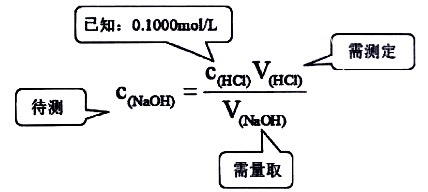
\includegraphics[max width=0.5\textwidth]{image/c1.jpg}
	\end{center}
	
	\subsection{滴定实验仪器以及操作要点}
	
	\subsubsection{滴定方法的关键}
	
	(1)准确测定两种反应物溶液的体积
	
	(2)确保标准液、待测液浓度的准确
	
	(3)\uline{滴定终点的准确判定}(包括指示剂的合理选用)
	\subsubsection{实验仪器及试剂}
	
	\begin{center}
		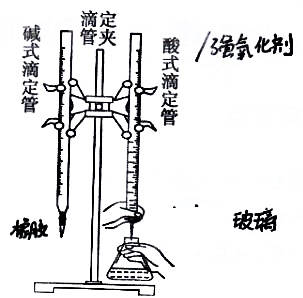
\includegraphics[max width=0.2\textwidth]{image/c2-1.jpg}
	\end{center}
	
	(1)仪器:酸式滴定管、碱式滴定管、滴定管夹、烧杯、锥形瓶、铁架台。
	
	\begin{center}
		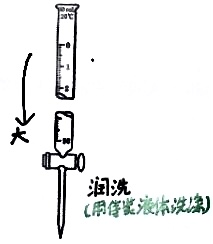
\includegraphics[max width=0.2\textwidth]{image/c2-2.jpg}
	\end{center}
	\[\mbox{酸式滴定管}\]
		\[\mbox{润洗--用待装液体洗涤}\]
	\begin{center}
		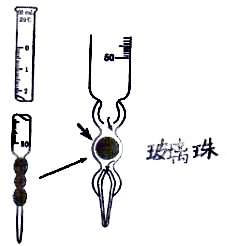
\includegraphics[max width=0.2\textwidth]{image/c2-3.jpg}
	\end{center}
		\[\mbox{碱式滴定管}\]
	 
	
	\subsubsection{滴定管的构造特点}
	
		\ding{172}标识: 标有温度、刻度、规格(25.00 mL 或 \({50.00}\mathrm{\;{mL}}\) )%圈1
	
	\ding{173}刻度:零刻度在\_\_\_,满刻度在\_\_\_;最小刻度为 0.1 ml,精确度为 0.01 ml。%圈2
	
	\ding{174}酸式滴定管: 下端是玻璃塞, 能盛装 \_溶液;
	
	碱式滴定管: 下端是橡皮管+玻璃小球, 能盛装\_
	
	%【思考 1】现在要量取 \({25.00}\mathrm{\;{mL}}\mathrm{{NaOH}}\) 溶液,应该用什么量取? 能不能用量筒? 为什么?
	
%	【思考 2】如图是某些仪器的刻度部分示意图, 图中各仪器虚线为所示读数。其中为量筒的是 \_\_\_(填编号,下同),读数为 \(2\text{、}n\mathrm{\;L}\) ;为滴定管的是\_\_\_,读数为 \(2\text{、}\mathrm{{SmL}}\)
	
%	\begin{center}
	%	\includegraphics[max width=0.3\textwidth]{images/0190d453-f338-754b-8cea-9ab8ce034fb0_0_605307.jpg}
	%\end{center}
	
%	① \ding{173}
	\subsubsection{凡士林的涂抹方式}
	
	\begin{center}
		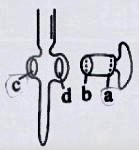
\includegraphics[max width=0.2\textwidth]{image/c3-1.jpg}
	\end{center}
	
		\[\mbox{涂a和c}\]
	
	
	润洗仪器: 在加入酸、碱之前, 洁净的酸式滴定管和碱式滴定管要分别用所要盛装的酸、碱润洗 \(2 \sim 3\) 次。
	
	\ding{173}方法是: 从滴定管上口加入 \(3 \sim 5\mathrm{\;{mL}}\) 所要盛装的酸溶液或碱溶液。倾斜着转动滴定管,使液体润湿全部滴定管内壁。然后, 一手控制活塞 (轻轻转动酸式滴定管的活塞; 或者轻轻挤压碱式滴定管中的玻璃球),将液体从滴定管下部放入预置的烧杯中。
	
	\ding{174}加入反应液: 分别将酸溶液、碱溶液加到酸式滴定管、碱式滴定管中,\uwave{ 使液面位于滴定管刻度“0”以上 \(2 \sim 3\mathrm{\;{mL}}\) 处},并将滴定管垂直固定在滴定管夹上。
	
	
	\ding{175}调节起始读数: 在滴定管下放一个烧杯, 调节活塞, 使滴定管尖嘴部分充满反应液, 并使液面处于“0”刻度(或“0”刻度以下),准确读取读数并记录$¥V_{\mbox{始}}$
	
	【思考 7】如果滴定管内出现气泡怎么排出气泡? 
	
	排气泡: 酸式滴定管 \(\rightarrow\)尖嘴部分朝上,碱式滴定管\(\rightarrow\)
	
	\begin{center}
		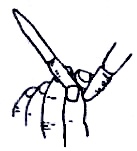
\includegraphics[max width=0.2\textwidth]{image/c4-1.jpg}
	\end{center}
		\[\mbox{除去碱式滴定管乳胶管中气泡的方法}\]
	
	
	\ding{176} 放液
	
	a 从碱式滴定管中放出 \({25.00}\mathrm{{ml}}\) 氢氧化钠溶液于锥形瓶中;
	
	
	
	\(\mathrm{b}\) 滴入几滴\uwave{酚酞试液}(指示剂),将锥形瓶置于酸式滴定管下方,并在瓶底衬一张白纸。
	
		\ding{177}滴定: 左手控制酸式滴定管活塞, 右手摇动锥形瓶, 边滴入盐酸 (当接近终点时, \uwave{改为滴加半滴酸}) , 边不断顺时针方向摇动, 眼睛要始终注视
	
	\begin{center}
		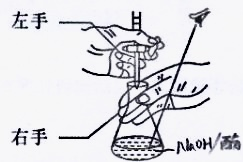
\includegraphics[max width=0.3\textwidth]{image/c4-2.jpg}
	\end{center}
	
	\ding{178}记读数: $\star$ \uwave{当滴入最后半滴HCl,溶液由红色突变为无色,且半分钟内不褪色. 停止滴定,准确记下盐酸读}数 \({\mathrm{V}}_{\text{终}}\) ,并准确求得滴定用去的盐酸体积 \(\mathrm{V} = {\mathrm{V}}_{\text{始 }} - {\mathrm{V}}_{\text{终 }}\) (平行实验 2 -3 次) 
	
	滴入最后半滴标准溶液具体操作?
	
	\ding{179}计算
	
	【经典 2】【2020 年 7 月选考】滴定前, 有关滴定管的正确操作为 (选出正确操作并按序排列,选项可重复使用): 检漏 \(\rightarrow\) 蒸馏水洗涤 \(\rightarrow\) 用滴定液润洗 2 至 3 次 \(\rightarrow\) 装入滴定液至零刻度以上 \(\rightarrow\) 排除气泡 \(\rightarrow\) 调整滴定液液面至零刻度或零刻度以下\( \rightarrow \)记录起始读数 \(\rightarrow\) 开始滴定。
	
	
\subsection{指示剂的选择}

\subsubsection{酸碱指示剂}

(1)酸碱指示剂的变色范围(pH 值) 

\begin{center}
	\adjustbox{max width=\textwidth}{
		\begin{tabular}{|c|c|c|c|}
			\hline
			\multirow{2}{*}{甲基橙} & \(< {3.1}\) & \({3.1} \sim {4.4}\) & \(> {4.4}\) \\
			\hline
			& 红 & 橙 & 黄 \\
			\hline
			\multirow{2}{*}{酚酞} & \(< {8.2}\) & \({8.2} \sim {10}\) & \(> {10}\) \\
			\hline
			& 无色 & 浅红 & 红 \\
			\hline
			\multirow{2}{*}{石蕊} & \(< 5\) & \(5 \sim 8\) & \(> 8\) \\
			\hline
			& 红 & 紫 & 蓝 \\
			\hline
		\end{tabular}
	}
\end{center}
\paragraph{滴定终点}

\[\mbox{显酸}\Rightarrow\mbox{甲基橙}\]
\[\mbox{显碱}\Rightarrow\mbox{酚酞}\]
\paragraph{变化曲线}

若以酸碱中和滴定过程中滴加酸 (或碱) 的量为横轴,以溶液的 \(\mathrm{{pH}}\) 为纵轴,即可绘出的一条溶液 \(\mathrm{{pH}}\) 随酸(或碱)的滴加量而变化的曲线。

\begin{center}
	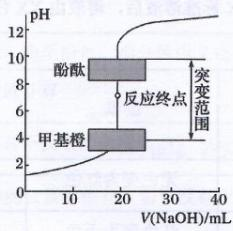
\includegraphics[max width=0.3\textwidth]{image/c5.jpg}
\end{center}

\subsection{小结}

\subsubsection{指示剂的选择原则}

①变色要明显、灵敏;

②指示剂的变色范围要尽可能在滴定过程中的 \(\mathrm{{pH}}\) 值突变范围内。

③指示剂用量不能太多, \(2 \sim 3\) 滴即可:

\subsubsection{指示剂的选择(由滴定曲线可知)}

①强酸强碱相互滴定, 可选用甲基橙或酚酞。

②若反应生成强酸弱碱盐, 溶液呈酸性, 则选用酸性变色范围的指示剂 (甲基橙);

若反应生成强碱弱酸盐, 溶液呈碱性, 则选用碱性变色范围的指示剂 (酚酞)

③石蕊试液因颜色变化不明显, 且变色范围过宽, 一般不作滴定指示剂。

④酸性 \({\mathrm{{KMnO}}}_{4}\) 溶液等本身呈现颜色的滴定试剂,不用另外选择指示剂

\subsubsection{终点判断}

 滴入最后半滴 XX 标准溶液后, 溶液由 XX 色突变 XX 色, 且半分钟内不褪色。

\begin{center}
	\adjustbox{max width=\textwidth}{
		\begin{tabular}{|c|c|c|}
			\hline
			指示剂 操作 & 酚酞 & 甲基橙 \\
			\hline
			强碱滴定强酸 & 无色变为红色 & 橙色变为黄色 \\
			\hline
			强酸滴定强碱 & 红色变为无色 & 黄色变为橙色 \\
			\hline
		\end{tabular}
	}
\end{center}

\subsection{误差分析}

以一元酸和一元碱的中的滴定为例

\[
{\mathrm{C}}_{\text{待 }}{\mathrm{V}}_{\text{待 }} = {\mathrm{C}}_{\text{标· }}{\mathrm{V}}_{\text{标 }}
\]

滴定过程中任何错误操作都有可能导致 \(\mathrm{C}\) 标、 \(\mathrm{V}\) 标、 \(\mathrm{V}\)待 的误差。但在实际操作中认为 \(\mathrm{C}\) 标是已

知的, \({\mathrm{V}}_{\text{待 }}\) 是固定的,对于 \({\mathrm{c}}_{\left( \mathrm{{NaOH}}\right) }  = \frac{{\mathrm{c}}_{\left( \mathrm{{HCl}}\right) }{\mathrm{V}}_{\left( \mathrm{{HCl}}\right) }}{{\mathrm{V}}_{(NaOH)} } \)


\[\mbox{读数比实际}\]

\subsection{误差分析}


\begin{center}
	\adjustbox{max width=\textwidth}{
		\begin{tabular}{|c|c|c|c|c|}
			\hline
			\phantom{X} & 产生误差的常见因素 & & 对 \(\mathrm{V}_{\mathrm{HCl}}\) 的影响 & 对 \(\mathbf{C}_{\mathrm{NaOH}}\) 的影响 \\
			\hline
			\multirow{4}{*}{滴定前操作} & 未用标准液润洗酸式滴定管 & [HCL]$\downarrow$& \(\uparrow\) & \(\uparrow\) \\
			\cline{2-5}
			& 未用待测液润洗碱式滴定管 &[NaOH]$\downarrow$& \(\downarrow\) & \(\downarrow\) \\
			\cline{2-5}
			& 用待测液润洗锥形瓶 &NaOH$\uparrow$& \(\uparrow\) & \(\uparrow\) \\
			\cline{2-5}
			& 洗涤后锥形瓶未干燥 &n(NaOH)不变& \(-\) & \(-\) \\
			\hline
			\multirow{2}{*}{滴定时读数不准} & 滴定前俯视酸式滴定管,滴定后平视 & & \(\uparrow\) & \(\uparrow\) \\
			\cline{2-5}
			& 滴定前仰视酸式滴定管,滴定后俯视&  & \(\uparrow\) & \(\uparrow\) \\
			\hline
			\multirow{2}{*}{取液时读数不准} & 取待测液时先俯视后仰视& & \(\downarrow\) & \(\downarrow\) \\
			\cline{2-5}
			& 取待测液时先仰视后俯视&  &\(\uparrow\) & \(\uparrow\) \\
			\hline
			\multirow{6}{*}{操作不当} & 滴定前酸式滴定管有气泡,滴定后气泡消失&  & \(\uparrow\) & \(\uparrow\) \\
			\cline{2-5}
			& 滴定前酸式滴定管无气泡,滴定后有气泡&  & \(\downarrow\) & \(\downarrow\) \\
			\cline{2-5}
			& 滴定结束,滴定管尖端挂一滴液体未滴下 & & \(\uparrow\) & \(\uparrow\) \\
			\cline{2-5}
			& 滴定过程中,振荡锥形瓶时,不小心将溶液溅出 & & \(\uparrow\) & \(\uparrow\) \\
			\cline{2-5}
			& 用甲基橙作指示剂,滴至橙色,半分钟内又还原成黄色,不处理就计算 & & \(\uparrow\) & \(\uparrow\) \\
			\cline{2-5}
			& 配制标准液的固体有不反应的杂质 & & \(\downarrow\) & \(\uparrow\) \\
			\hline
		\end{tabular}
}
\end{center}
%\end{comment}


\section{其他滴定}

\subsection{氧化还原滴定}

\subsubsection{酸性 \({\mathrm{{KMnO}}}_{4}\) 溶液滴定 \({\mathrm{H}}_{2}{\mathrm{C}}_{2}{\mathrm{O}}_{4}\) 溶液}

原理: \(2{\mathrm{{MnO}}}_{4}^{ - } + 6{\mathrm{H}}^{ + } + 5{\mathrm{H}}_{2}{\mathrm{C}}_{2}{\mathrm{O}}_{4} = {10}{\mathrm{{CO}}}_{2} \uparrow + 2{\mathrm{{Mn}}}^{2 + } + 8{\mathrm{H}}_{2}\mathrm{O}\) ;

指示剂及滴定终点: 酸性 \({\mathrm{{KMnO}}}_{4}\) 溶液本身呈紫红色,不用另外选择指示剂,当滴入最后半滴酸性 \({\mathrm{{KMnO}}}_{4}\) 溶液,溶液由无色变浅红色,且半分钟内不变色,说明达到滴定终点。

\subsubsection{ \({\mathrm{{Na}}}_{2}{\mathrm{\;S}}_{2}{\mathrm{O}}_{3}\) 溶液滴定碘液}

原理: \(2{\mathrm{\;S}}_{2}{\mathrm{O}}_{3}^{2 - } + {\mathrm{I}}_{2} = {\mathrm{S}}_{4}{\mathrm{O}}_{6}^{2 - } + 2{\mathrm{I}}^{ - }\) ;

指示剂及滴定终点: 用淀粉溶液+作指示剂,当滴入最后半滴 \({\mathrm{{Na}}}_{2}{\mathrm{\;S}}_{2}{\mathrm{O}}_{3}\) 溶液,溶液的蓝色褪去, 且半分钟内不恢复原色, 说明达到滴定终点。


\chapter{原电池}

\section{原电池}

\textit{将化学能转化为电能的装置, 本质为自发进行的氧化还原反应。}

\paragraph*{正极}

化合价$\downarrow$,得$e^{-}$$\Rightarrow$牺牲阳极的阴极保护法

\paragraph*{负极}

化合价$\uparrow$,失$e^{-}$,氧化反应

\subsection{原电池的构成条件}

1、活性不同的两极 
2、自发的氧化还原反应
3、闭合回路 
4、电解质

\section{盐桥}

\begin{center}
	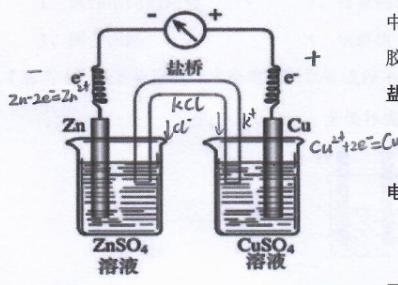
\includegraphics[max width=0.5\textwidth]{image/c14.jpg}
\end{center}

\subsection{盐桥构成}

盐桥里的物质一般是\dotuline{强电解质}而且不与两池中电解质反应, 常使用装有饱和 \(\mathrm{{KCl}}\) 琼脂溶胶的 \(\mathrm{U}\) 形管,离子可以在其中自由移动。

盐桥作用:

电极反应方程式: 

三大流向: 

\section{膜电池}

膜的引入简化了装置, 用离子交换膜分隔成两池, 仅允许特定的离子通过; 且膜能持续、长期使用。

\begin{center}
	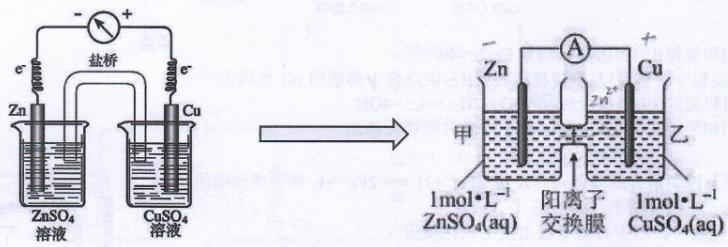
\includegraphics[max width=0.9\textwidth]{image/c16-1.jpg}
\end{center}

膜的分类:
 \textit{叫什么就只让什么离子过}

\ding{172}阳离子交换膜%圈1

\ding{173}阴离子交换膜

\ding{174}质子交换膜

只有$H^{+}$能过

\ding{175}双极膜

$H_{2}O\rightleftharpoons H^{+}+OH^{-}$一人去一边

\chapter{电解池}

%\section{电解池}

\begin{center}
	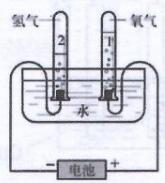
\includegraphics[max width=0.2\textwidth]{image/c19.jpg}
\end{center}

%请从电解水的能量变化和物质变换, 分析电解池的原理。

%\section*{电解池}

\textit{电解池: 把电能转变为化学能的装置。}

\paragraph*{构成条件}~{}\\

1.电源

2.两个电极(只导电,可用惰性电极--石墨,铂Pt,金Au)

3.电解质(水/熔融)

4.闭合回路

\paragraph*{两个电极}~{}\\

\subparagraph*{阳极}
失去$e^{-}$化合$\uparrow$ 氧化反应
\subparagraph*{阴极}
得$e^{-}$化合$\downarrow$ $\Rightarrow$\textbf{外加电源的阴极保护法}

\paragraph*{流向}

\subparagraph*{电子}

阳$\rightarrow$阴

\subparagraph*{电流}

阴$\rightarrow$阳

\subparagraph*{$\star$离子}

异性相吸(阳离子$\rightarrow$阴极)

\section{电极反应方程式书写}

电极反应式: 电化学装置中表示原子或离子在电极上得失电子发生氧化或还原反应的式子

\subsection{电极方程式的书写步骤}

1.确定主要反应物和生成物

2.得(阴)/失(阳)  $e^{-}$数

3.环境离子(电荷守恒)

4.元素守恒配齐($H_{2}O$)

\section{溶液中的离子放电顺序}

\textbf{$\textreferencemark$由于各种离子得失电子的能力不同, 因此, 电解时离子放电难易也不同。}

\subsection{阴极上阳离子放电}

\paragraph*{氧化性}~{}\\

$Ag^{+} > Hg^{+} > Fe^{3+} > Cu^{2+} > H^{+}(\mbox{酸}) > Sn^{2+} > Fe^{2+} > Zn^{2+} > H^{+}(\mbox{水})$

$>Al^{3+} > Mg^{2+} > Na^{+} > Ca^{2+} > K^{+}$

\[\text{有}Cu^{2+} Ag^{+} \text{出}Cu,Ag\]
\[\text{无}Cu^{2+} Ag^{+} \text{出}H_{2},\text{放氢生碱}OH^{-}\]

\subsection{阳极上阴离子放电}

\paragraph*{还原性}~{}\\
	
	金属电极(除Pt,Au) > $S^{2-} > {SO_{3}}^{2-} > I^{-} > Br^{-} > Cl^{-} > OH^{}(\text{水/碱})\rightarrow O_{2}$
	
	
	>最高价含氧酸根${SO_{4}}^{2-},{CO_{3}}^{2-},{NO_{3}}^{-} > F^{-}$ 
	
	\[\text{有卤素出卤素}\]
	\[\text{无卤素出}O_{2},\text{放氧生酸}H^{+}\]
	
	
	
	% 定义 longtable 环境,表格有 4 列,每列内容居中对齐并用竖线分隔
	\begin{longtable}{|c|c|c|c|} 
		
		\hline % 表格顶部的横线
		
		% 表头部分
		\textbf{电解池情况} & \textbf{阳极产物} & \textbf{阴极产物} & \textbf{阳极: 阴极产物比例} \\ % 表头行,加粗列标题
		\hline % 表头行的下横线
		\endfirsthead % 结束表头部分的定义
		
		% 如果表格跨页,表头重复部分
		\hline % 表头行的上横线
		\textbf{电解池情况} & \textbf{阳极产物} & \textbf{阴极产物} & \textbf{阳极: 阴极产物比例} \\ % 表头行,加粗列标题
		\hline % 表头行的下横线
		\endhead % 结束表头重复部分的定义
		
		% 表格主体的底部横线
		\hline
		\endfoot % 结束表格主体的底部横线部分
		
		% 表格最后一页的底部横线
		\hline
		\endlastfoot % 结束表格最后一页的底部横线部分
		
		% 表格内容部分
		a.b 为铂电极, 硫酸钠溶液 & $O_{2}$ & $H_{2}$ & 1:2 \\ % 第一行数据
		\hline % 每行数据之后加横线
		a.b 为铂电极,硫酸铜溶液 & $O_{2}$ & Cu & 1:2 \\ % 第二行数据
		\hline
		a.b 为铂电极, 氯化铜溶液 & $Cl_{2}$ & Cu & 1:1\\ % 第三行数据
		\hline
		a, b 为铂电极,氯化钠溶液 & $Cl_{2}$ & $H_{2}$ & 1:1 \\ % 第四行数据
		\hline
		a, b 为铁电极, 氯化钠溶液 & $Fe^{2+}$ & $H_{2}$ & 1:1 \\ % 第五行数据
		\hline
	%	行6 & 数据16 & 数据17 & 数据18 \\ % 第六行数据
	%	\hline
		
	\end{longtable} % 结束 longtable 环境
	
	\subsection{阶段放电}
	
	$
	
	\left\{
	\begin{aligned}
		\text{足量XX溶液} \Rightarrow  	\text{无阶段(看溶液)} \\
		\text{少量/一定量XX溶液} \Rightarrow  	\text{顺序} \\
	\end{aligned}
	\right.
	$
	
	
	\section{电解池中膜的应用}
	
	
	\begin{center}
		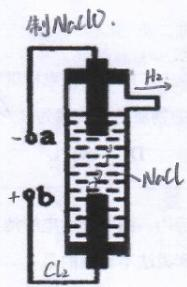
\includegraphics[max width=0.2\textwidth]{image/c26-1.jpg}
	\end{center}
	
	
	\begin{center}
	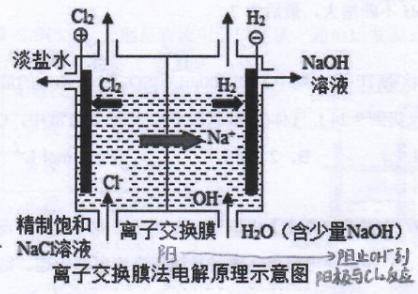
\includegraphics[max width=0.5\textwidth]{image/c26-2.jpg}
	\end{center}
	
	
	\subsection{离子交换膜}
	
	工业上氯碱工业利用离子交换膜来制备氯气和氢氧化钠;
	
	工业上利用离子交换膜进行\uwave{废水处理、海水淡化}等。
	
\section{二次电池}

二次电池又称可充电电池或蓄电池放电后可以充电使活性物质获得再生, 此类电池可重复使用。

\subsection{铅酸蓄电池}

稀硫酸

\({\mathrm{{PbO}}}_{2}\) (正极)

\(\mathrm{{Pb}}\) (负极)

放电时的电极方程式:

负极: \(\mathrm{{Pb}} + {\mathrm{{SO}}}_{4}{}^{2 - } - 2\mathrm{e} = {\mathrm{{PbSO}}}_{4}\)

正极: \({\mathrm{{PbO}}}_{2} + 4{\mathrm{H}}^{ + } + {\mathrm{{SO}}}_{4}{}^{2 - } + 2\mathrm{e} - = {\mathrm{{PbSO}}}_{4} + 2{\mathrm{H}}_{2}\mathrm{O}\)

总反应: \(\mathrm{{Pb}} + {\mathrm{{PbO}}}_{2} + 2{\mathrm{H}}_{2}{\mathrm{{SO}}}_{4} = 2{\mathrm{{PbSO}}}_{4} + 2{\mathrm{H}}_{2}\mathrm{O}\)

$\longleftarrow$电解池

\paragraph*{阳极}

$PbSO_{4} - 2e^{-} +2H_{2}O = PbO_{2} + 4H^{+} + {SO_{4}}^{2-}$
	\[\mbox{正接正(阳),负接负(阴)}\]
	\[\mbox{电极方程式完全相反},e^{-}\mbox{换边}\]
	
\subsection{锂离子电池}

 质量小、体积小、储存和输出能量大 (合金)
负极材料: 嵌锂石墨 正极材料: \({\mathrm{{LiCoO}}}_{2}\) (钴酸锂)

电解质溶液为 \({\mathrm{{LiPF}}}_{6}\) (六氟磷酸锂) 的碳酸酯溶液 (无水)

放电过程总反应为: \({\mathrm{{Lix}}}C\mathrm{y} + {\mathrm{{Li}}}_{1 - \mathrm{x}}{\mathrm{{CoO}}}_{2} \rightarrow {\mathrm{{LiCoO}}}_{2} + \mathrm{{Cy}}\)


\paragraph*{负极}

: \(\mathrm{{LixCy}} - \mathrm{{xe}} = {\mathrm{{xLi}}}^{ + } + \mathrm{{Cy}}\) 
\[{Li - {e}^{ - } = Li^{ + }\]

\paragraph*{正极}

 \({\mathrm{{Li}}}_{1 - \mathrm{x}}{\mathrm{{CoO}}}_{2} + {\mathrm{{xLi}}}^{ + } + {\mathrm{{xe}}}^{ - } = {\mathrm{{LiCoO}}}_{2}\) 
\[{\mathrm{{Li}}}^{ + } + {\mathrm{e}}^{ - } = \mathrm{{Li}}\]


\section{原电池与电解池的串联}

原电池电解池的串联: 利用原电池放电来作为电解池的电源。

	\[\mbox{先找原电池}\Rightarrow \mbox{电极活泼性/气体}\]
	\[\mbox{跨膜电子数}= \mbox{转移} e^{-}\]
	
	
	
\part{物质结构与性质}

\chapter{原子结构}
	

\section{原子构造原理发展历史}

\begin{center}
	\adjustbox{max width=\textwidth}{
		\begin{tabular}{|c|c|c|c|}
			\hline
			年份 & 国籍 & 科学家 & 贡献 \\
			\hline
			1814 年 & 德国 & 夫琅禾费 & 发明分光镜, 观察太阳光, 发现夫琅禾费线 \\
			\hline
			1859 年 & 德国 & 本生、基尔霍夫 & 证明夫琅禾费线是原子的吸收光谱, \\
			\hline
			1869 年 & 俄国 & 门捷列夫 & 发现元素周期表 \\
			\hline
			1913 年 & 丹麦 & 波尔 & 提出氢原子模型:电子在线性轨道绕核运行 \\
			\hline
			1918 年 & 丹麦 & 波尔 & 提出“能层”与“能级” \\
			\hline
			1920 年 & 丹麦 & 波尔 & 提出构造原理 \\
			\hline
			1926 年 & \multicolumn{3}{|c|}{量子力学} \\
			\hline
			1936 年 & 德国 & 马德隆 & 发表完整的构造原理 \\
			\hline
		\end{tabular}
	}
\end{center}

	
	\section{能层与能级}
	
	\paragraph*{能层}: 核外电子按照能量不同分成能层, \textit{能层越高, 电子离核越远, 电子的能量越高。}
	
	\begin{center}
		\adjustbox{max width=\textwidth}{
			\begin{tabular}{|c|c|c|c|c|c|c|c|}
				\hline
				能层 & 一 & 二 & 三 & 四 & 五 & 六 & 七 \\
				\hline
				符号 & \(\mathrm{K}\) & L & M & \(\mathrm{N}\) & O & P & Q \\
				\hline
				最多电子数 & 2 & 8 & 18 & 32 & 50 & 72 & 98 \\
				\hline
			\end{tabular}
		}
	\end{center}
	
	能量的高低顺序为: \(\mathrm{E}\left( \mathrm{K}\right) < \mathrm{E}\left( \mathrm{L}\right) < \mathrm{E}\left( \mathrm{M}\right) < \mathrm{E}\left( \mathrm{N}\right) < \mathrm{E}\left( \mathrm{O}\right) < \mathrm{E}\left( \mathrm{P}\right) < \mathrm{E}\left( \mathrm{Q}\right)\) 。
	
	能层=电子层
	
\paragraph*{能级}: 同一能层的电子, 还被分为不同能级, 每一能级所能容纳的电子数目也不同。能级的符号
	和所能容纳的最多电子数如下:
	
	\begin{center}
		\adjustbox{max width=\textwidth}{
			\begin{tabular}{|c|c|c|c|c|c|c|c|c|c|c|c|c|}
				\hline
				能层 & \(\mathbf{K}\) & \multicolumn{2}{|c|}{L} & \multicolumn{3}{|c|}{\(\mathbf{M}\)} & \multicolumn{4}{|c|}{\(\mathbf{N}\)} & \multicolumn{2}{|c|}{\(\mathbf{O}\)} \\
				\hline
				能 级 & 1s & 2s &2p & 3s &  3p & 3d &4s & 4p & 4d & 4f & 5s & 5p  \\
				\hline
				最多 电子数 & 2 & 2 &  6&  2&  6  & 10 &  2 & 6 & 10 & 14 &   2 & 6  \\
				\hline
			\end{tabular}
		}
	\end{center}
	
	\subparagraph*{s} $ 1 \times 2 $
	
	\subparagraph*{p} $ 3 \times 2 $
	
	\subparagraph*{d} $ 5 \times 2 $
	
	\subparagraph*{f} $ 7 \times 2 $
	
	
	\textit{能层数=具有的能级数}
	
\subsection{同能级比能层}
\[ns>(n-1)s>(n-2)s>(n-3)s\]

\section{构造原理和电子排布式}

\subsection{构造原理}
	
	以光谱学事实为基础, 从氢开始, 随核电荷数递增, 新增电子填入能级的顺序称为构造原理。
	
	\begin{center}
		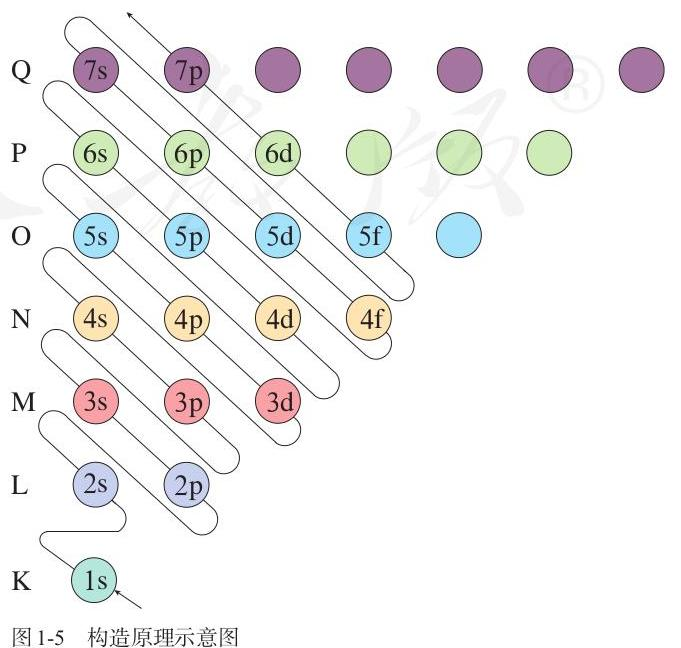
\includegraphics[max width=0.5\textwidth]{image/c43-2.jpg}
	\end{center}
	
	\subsection{能级交错}
	\paragraph*{原理:} 电子总是占据能量较低的能级。
	
	\paragraph*{影响因子 1:} 占据能量较 高能级使整体能量升高。
	
	\paragraph*{影响因子 2: }同一能级电子排斥使整体能量升高。
	
	\textit{当相邻两个能级能量相差不大, 电子排斥能大于两个能级之间能量差距, 电子填充能量较高能级, 出现能级交错。}
		\begin{center}
		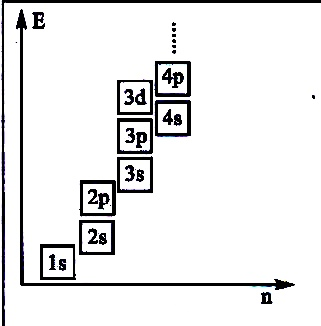
\includegraphics[max width=0.5\textwidth]{image/c43-1.jpg}
	\end{center}
	
	
	按照构造原理, 电子填满一个能级, 开始填入下一个能级, 由此构建了元素周期表中各元素的基态原子的电子排布。
	
		\begin{center}
		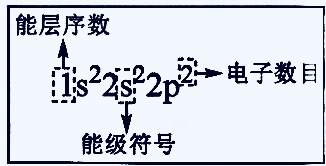
\includegraphics[max width=0.3\textwidth]{image/c44.jpg}
	\end{center}
	
	
	4s<3d能量
	
			$
	
	\left\{
	\begin{aligned}
		\text{书写:先3d再4s}  \\
		\text{得失}e^{-}   \text{先4s再3d}\\
	\end{aligned}
	\right.
	$
	
	\subsection{屏蔽效应}
	
	由于其他电子对某一电子的排斥作用而抵消了一部分核电荷对该电子的吸引力. 从而引起有效核电荷的降低, 削弱了核电荷对该电子的吸引, 这种作用称为屏蔽作用或屏蔽效应。
	
	\paragraph*{价电子层}在化学反应中可能发生电子变动的能级称为价电子层 (简称价层)。
	\paragraph*{简化电子排布式} [前一周期稀有气体符号]价层电子排布。 (3d不含在Ar里面)
	
	\section{基态与激发态原子光谱}
	
	\paragraph*{基态原子:} 处于最低能量状态的原子叫做基态原子。
	
	\paragraph*{激发态原子:} 基态原子吸收能量, 它的\uwave{电子会跃迁到较高能级}(\uline{只能跳到相邻层级}), 变为激发态原子。
	
	电子从较高能量的激发态跃迁到较低能量的激发态乃至基态时, 将释放能量 (主要以光的形式)。
	
	\subsection{原子光谱}
	
	不同元素原子的电子发生跃迁时会吸收或释放不同的光, 可以用光谱仪摄取各种元素原子的吸收光谱或发射光谱, 总称原子光谱。
	\subsubsection{原子吸收光谱}
	
	电子由低能级向高能级发生跃迁, 会吸收一定波长的光线, 因此会在全光谱上留下相应的暗线, 称为原子吸收光谱。
	
	基 \(  \rightarrow   \) 激
	
	\subsubsection{原子发射光谱}
	
	电子由高能级向低能级发生跃迁, 会释放一定波长的光线, 称为原子发射光谱。
	
	在现代化学中, 常利用原子光谱上的特征谱线来鉴定元素, 称为光谱分析。
	
	激$\rightarrow$基  焰色试验
	\subsubsection*{日常应用}
	
	 焰火、霓虹灯光、激光、萤光、LED 灯光等。
	 
\chapter{电子云与原子轨道}
	 
	 概率密度: 用 \(\mathrm{P}\) 表示电子在某处出现的概率, \(\mathrm{V}\) 表示该处的体积,则 \(\mathrm{P}/\mathrm{V}\) 称为概率密度,用 \(\rho\) 表示。
	 
	 	\begin{center}
	 	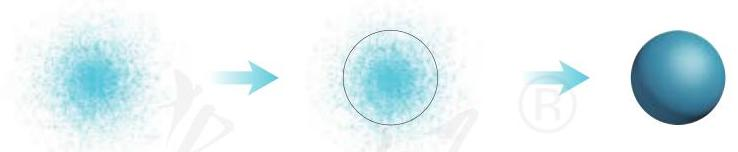
\includegraphics[max width=0.5\textwidth]{image/c51-1.jpg}
	 \end{center}
	 \section{电子云 }
	 
	 由于核外电子的\uwave{概率密度分布}看起来像一片云雾, 因而被形象地称作电子云。
	 
	 \section{电子云轮廓图}
	 
	 把电子在原子核外空间出现概率 \(\mathrm{P} = {90}\%\) 的空间圈出来,得到电子云轮廓图。 
	 
	 \section{电子云轮廓图形状}
	 
	\subsection{s电子云轮廓图}
	
	 \uwave{球形},且能层序号越大,半径越大。
	 
	 	\begin{center}
	 	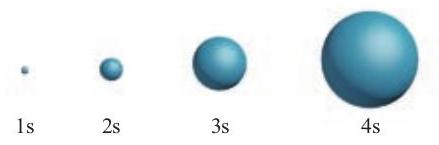
\includegraphics[max width=0.5\textwidth]{image/c51-2.jpg}
	 \end{center}
	 
	 \subsection{p 电子云轮廓图} 
	 
	 \uwave{哑铃形},且有三个互相垂直的电子云
	 
	 $P_{x},P_{y},P_{z}$能量相同
	 
	 	\begin{center}
	 	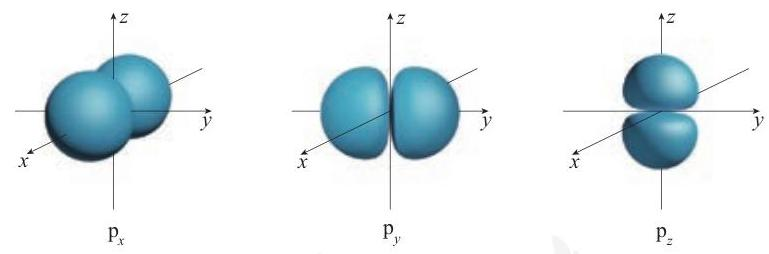
\includegraphics[max width=0.5\textwidth]{image/c51-3.jpg}
	 \end{center}
	 
	 \section{钻穿效应} 
	 
	 在原子核附近出现的概率较大的电子, 可更多地避免其余电子的排斥, 受到核的较强的吸引而更靠近核, 这种进入原子内部空间的作用叫做钻穿效应, 钻穿效应可以使能级降低。
	 
	 \section{原子轨道}
	 
	 量子力学把电子在原子核外的一个空间运动状态称为一个原子轨道。
	 
	 每一个轨道最多容纳两个电子, \(\mathrm{s}\) 能级包含 1 个轨道, \(\mathrm{p}\) 能级包含 3 个轨道, \(\mathrm{d}\) 能级包含 5 个轨道, \(f\) 能级包含 7 个轨道
	 
	 \begin{center}
	 	\adjustbox{max width=\textwidth}{
	 		\begin{tabular}{|c|c|c|c|c|}
	 			\hline
	 			能级 & ns & np & nd & nf \\
	 			\hline
	 			轨道数目 & 1 & 3 & 5 & 7 \\
	 			\hline
	 			最多容纳电子数 & 2 & 6 & 10 & 14 \\
	 			\hline
	 		\end{tabular}
	 	}
	 \end{center}
	 
	 \chapter{泡利原理、洪特原理、能量最低原理}
	 
	 轨道表示式: 用方框 (也可用圆圈) 表示原子轨道, 能量相同的原子轨道称为简并轨道。
	 
	 自旋: 电子除空间运动状态外, 还有一种状态叫自旋。电子自旋在空间有顺时针和逆时针两种取向,简称自旋相反,常用上下箭头 \(\left( { \uparrow \text{和} \downarrow }\right)\) 表示自旋相反的电子。
	 
	 \section{ 洪特规则}
	 \textit{ 基态原子中, 填入简并轨道的电子总是\uwave{先单独分占, 且自旋平行}, 称为洪特规则。}
	  
	  	 \begin{center}
	  	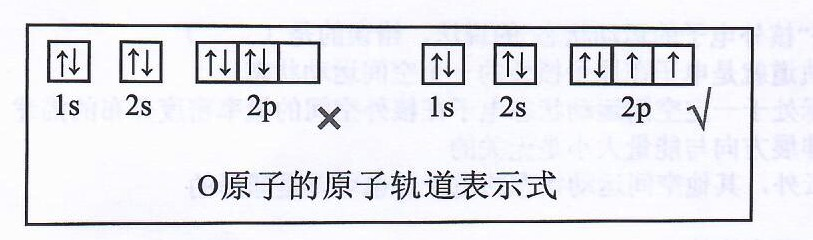
\includegraphics[max width=0.6\textwidth]{image/c54-1.jpg}
	  \end{center}
	  
	 \section{泡利原理}
	 
	 \textit{\uwave{在一个原子轨道里, 最多只能容纳两个电子, 他们的自旋相反}, 这个原理被称为泡利原理。}
	
	 	 \begin{center}
	 	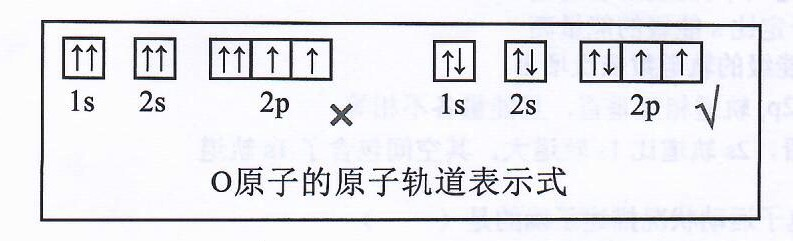
\includegraphics[max width=0.6\textwidth]{image/c54-2.jpg}
	 \end{center}

	 
	 \section{能量最低原理}
	 
	  \textit{在构建基态原子时, 电子将尽可能占据能量最低的原子轨道, 使整个原子的能量最低,这就是能量最低原理。 }
	  
	  \textbf{\textit{半满/全满 能量最低}}
	 
	 \begin{center}
	 	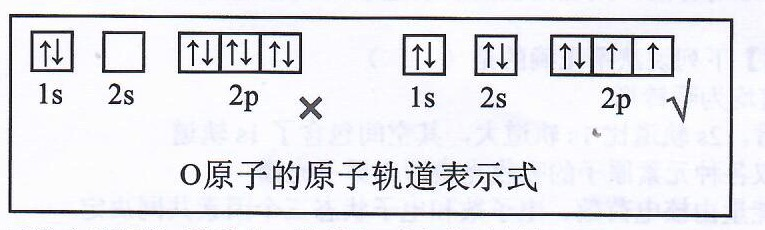
\includegraphics[max width=0.6\textwidth]{image/c54-3.jpg}
	 \end{center}
	 
	 \textit{基态原子的核外电子排布遵循泡利原理、洪特规则和能量最低原理。}
	 
	 
 \chapter{元素的性质}
	 
	 \section{元素周期表发展史}
	 
	 元素周期律: 元素的性质随元素原子的核电荷数递增发生周期性递变的规律。
	 
	 元素周期系: 元素按其原子核电荷数递增排列的\textbf{序列}称为元素周期系。
	 
	 元素周期表: 元素根据核电荷数从小至大排序的化学元素\textbf{列表}。元素周期系只有一个, 元素周期表多种多样。
	 
	 1869 年, 门捷列夫制作了历史上第一张元素周期表, 又称短式周期表。
	 
	 特征:从第四周期开始分为主副族,第八族称为过渡元素
	 
	 至今, 仍在使用第八族和主副族等名词, 但是概念已经有所不同。
	 
	 维尔纳周期表
	 
	 1905 年, 配位化学鼻祖维尔纳制作了一张元素周期表, 是一张特长式周期表, 每个周期一行, 每一个元素都有各自的位置, 同族元素上下对齐。
	 
	  波尔元素周期表
	 
	 1922 年, 波尔获诺贝尔奖时做了题为“原子结构”的报告, 其中包含的元素周期表。
	 
	 波尔已知镧 (La) 后 14 种元素基态原子有 \(4\mathrm{f}\) 电子,并用方框框起。
	 
	 波尔周期表还用直线连接前后相关元素, 因为波尔已经知道, 他们的价电子数相等。
	 
	 根据构造原理得出的核外电子排布, 可以解释元素周期系的基本结构。例如可以确定元素周期系中每个周期的元素数。
	 
	 除了第一周期以外,每个周期都是从 \(\mathrm{{ns}}\) 能级开始,以 \(\mathrm{{np}}\) 能级结束,而从 \(\mathrm{{ns}}\) 能级开始以 \(\mathrm{{np}}\) 能级结束递增的核电荷数就等于每个周期里的元素数。
\begin{comment}
		 \begin{center}
		\adjustbox{max width=\textwidth}{
			\begin{tabular}{|c|c|c|c|c|c|c|c|}
				\hline
				\phantom{X} & \phantom{X} & \phantom{X} & \phantom{X} & \phantom{X} & \phantom{X} & \(\mathrm{s}\mathrm{j} * \mathrm{{2s}} + 2\mathrm{p} * 2\mathrm{s} + 3\mathrm{p}\mathrm{j} * 4\mathrm{s} + 3\mathrm{d} + 4\mathrm{p} * 5\mathrm{s} + 4\mathrm{d} + 5\mathrm{p} * 6\mathrm{s} + 4\mathrm{f} + 5\mathrm{d} + 6\mathrm{p} * 7\mathrm{s} - 5\mathrm{f} + 6\mathrm{d} + 7\mathrm{p} - 5\mathrm{f} + 6\mathrm{d} + 7\mathrm{p} * \cdots\) & \phantom{X} \\
				\hline
				周期 & \(\rightarrow\) & 二 & 三 & 四 & 五 & 六 & 七 \\
				\hline
				元素数 & 2 & 8 & 8 & 18 & 18 & 32 & 32 \\
				\hline
			\end{tabular}
		}
	\end{center}
\end{comment}	 


\section{元素周期表的分区}

\begin{center}
	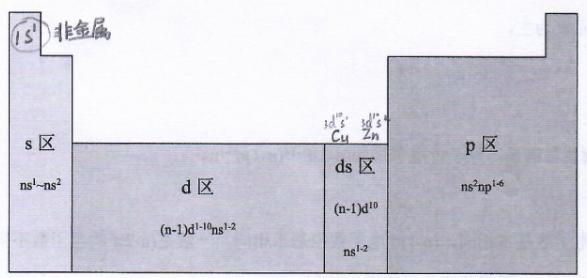
\includegraphics[max width=0.8\textwidth]{image/c61-1.jpg}
\end{center}

\begin{center}
	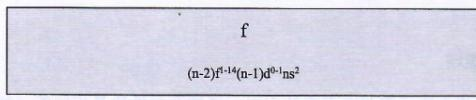
\includegraphics[max width=0.6\textwidth]{image/c61-2.jpg}
\end{center}

\(\mathrm{s}\) 区: 含IA 与IIA 共两族两列,原子价电子层为 \({\mathrm{{ns}}}^{1} \sim {\mathrm{{ns}}}^{2}\) 。

\(\mathrm{s}\) 区元素特征:

\ding{172} 价电子数 \(=\) 主族序数 \(=\) 最外层电子数;

\ding{173} 最外层电子数始终在 1-2 个,表现出较强的失电子能力,所以除 \(\mathrm{H}\) 外,都是金属元素。

d区: 含IIIB 至VIIB 和VIII族共六族八列,原子价电子层为 \(\left( {\mathrm{n} - 1}\right) {\mathrm{d}}^{1 - {10}}{\mathrm{{ns}}}^{1 - 2}\) 。

\(\mathrm{d}\) 区元素特征:

\ding{172} 价电子总数 \(=\) 副族序数,价电子总数为 8、9、10 个的为第 VIII 族;

\ding{173} 一般最外层电子数始终为 1-2 个 (Pd 是 18 个), 因此也容易失去电子, d 区元素都是金属元素。

\(\mathrm{{ds}}\) 区: 含IB 与IIB 共两族两列,原子价电子层为 \(\left( {\mathrm{n} - 1}\right) {\mathrm{d}}^{10}{\mathrm{{ns}}}^{1 - 2}\) 。

ds 区元素特征:

\ding{172} 最外层电子数 \(=\) 副族序数;

\ding{173} 均为金属元素; 且 \(\mathrm{d}\) 轨道电子全充满,一般不参与化学键的形成。

\(\mathrm{p}\) 区:含IIIA 至VIIA 及零族共六族六列,原子价电子层为 \(\mathrm{n{s}^{2}n{p}^{1 - 6}}\) 。

\(\mathrm{p}\) 区元素特征:

\ding{172}价电子总数 \(=\) 主族序数 (零族除外);

\ding{173}以非金属元素为主。

f 区 : 包括镧系与锕系,原子价电子层为 \(\left( {\mathrm{n} - 2}\right) {\mathrm{f}}^{1 - {14}}\left( {\mathrm{n} - 1}\right) {\mathrm{d}}^{0 - 1}{\mathrm{{ns}}}^{2}\)

\(\mathrm{f}\) 区元素特征:

由于最外层电子数基本相同, \(\left( {\mathrm{n} - 1}\right) \mathrm{d}\) 电子数也基本相同,一般是 \(\left( {\mathrm{n} - 2}\right) \mathrm{f}\) 的电子数不同,因此镧系元素化学性质相似; 锕系元素化学性质也相似。

\subsection{对角线规则}

在元素周期表中, 某些主族元素与右下方的主族元素的有些性质是相似的 (如锂和镁在过量的氧气中燃烧均生成正常氧化物, 而不是过氧化物), 这种相似性被称为对角线规则。

\section{元素周期律}

\subsection{原子半径}

原子半径的大小取决于两个相反的因素:

①电子的能层数: 电子的能层越多, 电子之间的排斥作用将使原子的半径增大;

②核电荷数: 核电荷数越大, 核对电子的吸引作用也越大, 将使原子的半径减小。

这两个因素综合的结果使原子半径呈现周期性的递变。

\begin{center}
	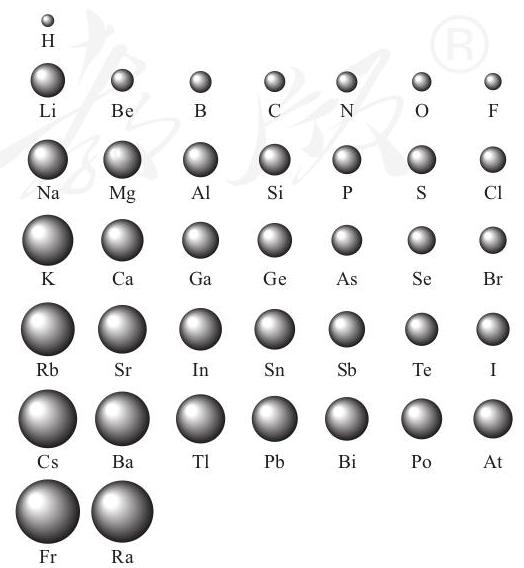
\includegraphics[max width=0.3\textwidth]{image/c65.jpg}
\end{center}

\subsection{电离能}

\textbf{第一电离能}: 气态电中性\uwave{基态原子}失去一个电子转化为气态基态正离子所需的最低能量叫做第一电离能。

$\Rightarrow$趋势与非金属性一致
\setcounter{num}{2}
$$\text{\Roman{num}}_{A},V_{A} \text{欺负邻居}$$



\begin{center}
	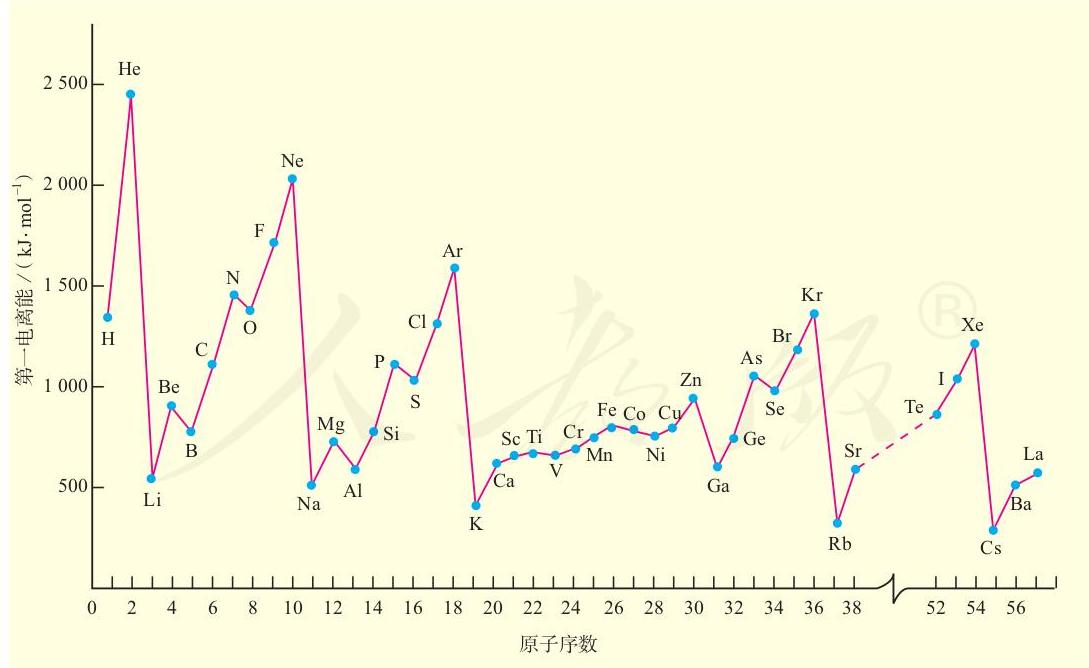
\includegraphics[max width=1.0\textwidth]{image/c66.jpg}
\end{center}

元素的第一电离能的周期性

第一电离能随核电荷数递增规律:

①同周期元素从左往右第一电离能增大 (并不是所有元素都遵循规律), 第一种元素第一电离能最小, 最后一种元素(稀有气体元素)第一电离能最大。

②同族元素从上到下第一电离能变小。(\textbf{\textit{找突变点,为常见价态}})

\begin{center}
	\adjustbox{max width=\textwidth}{
		\begin{tabular}{|c|c|c|c|}
			\hline
			元素 & Na & Mg & Al \\
			\hline
			\multirow{7}{*}{电离能 \(\mathrm{{kJ}} \cdot {\mathrm{{mol}}}^{-1}\)} & 496 & 738 & 578 \\
			\cline{2-4}
			& 4562 & 1451 & 1817 \\
			\cline{2-4}
			& 6912 & 7733 & 2745 \\
			\cline{2-4}
			& 9543 & 10540 & 11575 \\
			\cline{2-4}
			& 13353 & 13630 & 14830 \\
			\cline{2-4}
			& 16610 & 17995 & 18376 \\
			\cline{2-4}
			& 20114 & 21703 & 23293 \\
			\hline
		\end{tabular}
	}
\end{center}

\subsection{电负性}

\textbf{键合电}子: 原子中用于形成化学键的电子称为键合电子。

\textbf{电负性}: 描述不同原子对键合电子吸引力的大小。电负性越大的原子对键合电子的吸引力越大。

$\Rightarrow $氧化性$\Rightarrow$ 趋势与非金属性完全一致


\textbf{电负性标准:} 以氟的电负性为 4.0 , 锂的电负性为 1.0 。

电负性递变规律:

①同周期元素从左到右, 元素的电负性逐渐变大;

②同族元素从上到下, 元素的电负性逐渐变小。

\begin{center}
	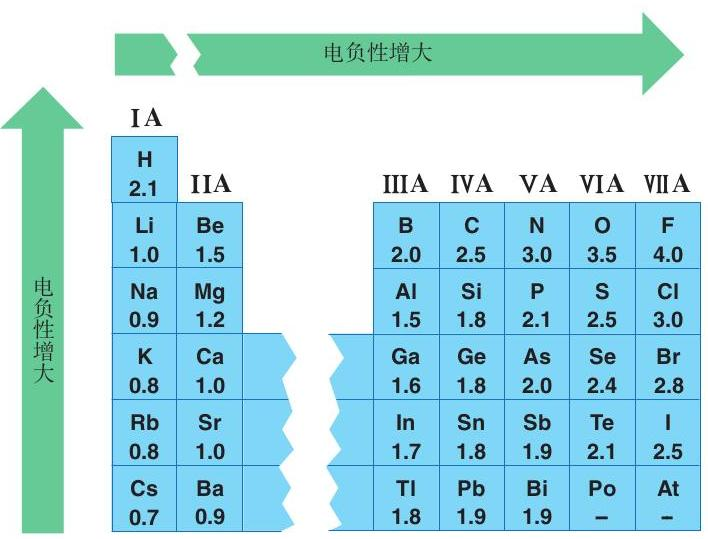
\includegraphics[max width=1.0\textwidth]{image/c68.jpg}
\end{center}

电负性的大小也可以作为判断金属性和非金属性强弱的依据:

①金属元素的电负性一般小于 1.8

②非金属元素的电负性一般大于 1.8

③处于金属和非金属交界线边缘的元素, 电负性在 1.8 左右, 既有金属性又有非金属性。

\chapter{共价键}

\section{共价键}

共价键是原子间通过共用电子对所形成的相互作用。

共价键具有饱和性,因此只能有 \({\mathrm{H}}_{2}\text{、}\mathrm{{HCl}}\text{、}{\mathrm{{Cl}}}_{2}\) 。不可能有 \({\mathrm{H}}_{3}\text{、}{\mathrm{H}}_{2}\mathrm{{Cl}}\) 和 \({\mathrm{{Cl}}}_{3}\) 等。

\begin{center}
	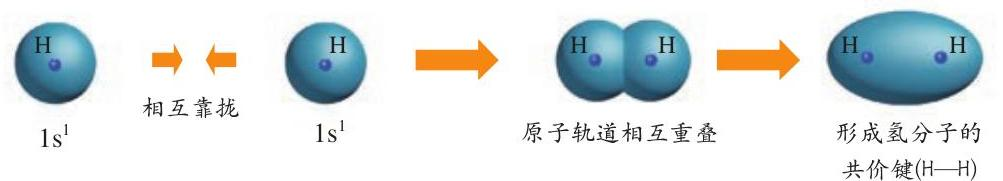
\includegraphics[max width=0.7\textwidth]{image/c72-1.jpg}
\end{center}

原子轨道在两个原子间重叠, 意味着电子出现在核间的概率变大, 电子对带正电荷的原子核有吸引作用, 使得两个原子结合在一起, 形成共价键。原子轨道的重叠程度越大, 共价键越牢固。

像这样两个原子轨道“\uwave{头碰头}”形成的共价键称为 \uwave{\(\sigma\) 键}。 \(\sigma\) 键的特征是以形成化学键的两原子核的连线为轴做旋转操作, 共价键的电子云的图形不变, 这种特征称为\uwave{\textbf{轴对称}}。(单键)

\({\mathrm{H}}_{2}\) 中的 \(\sigma\) 键是由两个 \(\mathrm{s}\) 轨道重叠形成的,可称为 \(\mathrm{s} - \mathrm{s}\sigma\) 键。 \(\mathrm{s}\) 轨道和 \(\mathrm{p}\) 轨道、 \(\mathrm{p}\) 轨道和 \(\mathrm{p}\) 轨道之间也可以重叠形成 \(\sigma\) 键。比如 \(\mathrm{{HCl}}\) 和 \({\mathrm{{Cl}}}_{2}\) 之间的共价键。

\begin{center}
	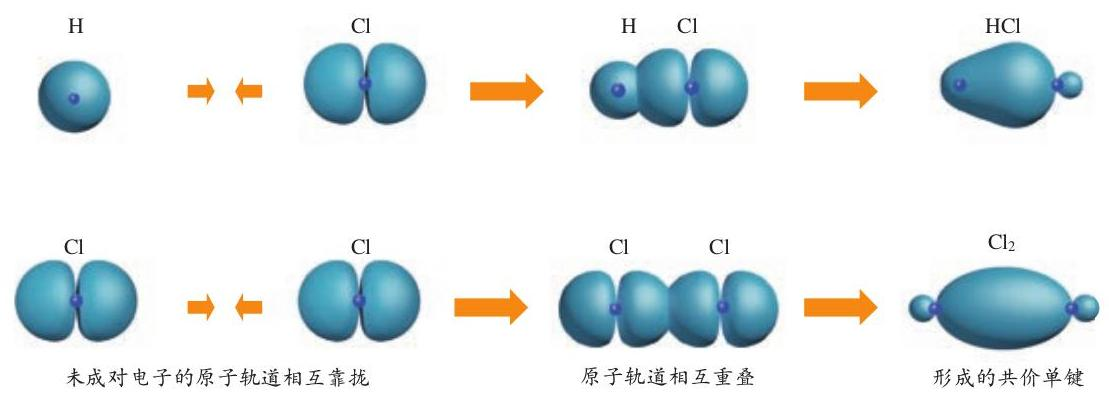
\includegraphics[max width=0.7\textwidth]{image/c72-2.jpg}
\end{center}

\(\mathrm{p}\) 轨道和 \(\mathrm{p}\) 轨道之间除了能够“头碰头”形成 \(\sigma\) 键之外还能“\uwave{肩并肩”形成 \(\pi\) 键}。 \(\pi\) 键的特征是电子云由互为镜像的两块电子云组成, 这种特征称为\uwave{\textbf{镜面对称}}。(\textit{二/三里面的第三根键})

\begin{center}
	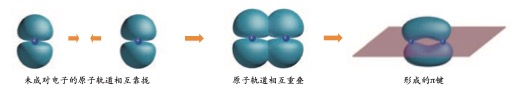
\includegraphics[max width=0.7\textwidth]{image/c73.jpg}
\end{center}

在形成化学键的过程中,一定是优先头碰头形成 \(\sigma\) 键,再肩并肩形成 \(\pi\) 键。

\(\pi\) 键和 \(\sigma\) 键的强度不同,一般情况下, \textit{\uwave{\(\sigma\) 键的强度要强于 \(\pi\) 键}}($\ce{N#N}$ $\sigma $弱于$\pi$)。例如在乙烯和乙炔中的 \(\pi\) 键强度不如 \(\sigma\) 键,容易断裂,因此含有 \(\pi\) 键的乙烯、乙炔的性质和只含 \(\sigma\) 键的乙烷的性质有较大的区别。

\chapter{分子的空间结构}

\section{分子结构的测定}

\subsection{ 红外光谱仪}

\textbf{原理}: 分子中的原子是在不停的振动的。当一束红外线透过分子时, 分子会吸收和它的某些化学

键的振动频率相同的红外线, 记录到图谱上呈现吸收峰。

通过和已有图谱库进行比对,或通过量子化学计算,可以得知各吸收峰是\textbf{由哪种化学键引起的}.($\Rightarrow$官能团)

\begin{center}
	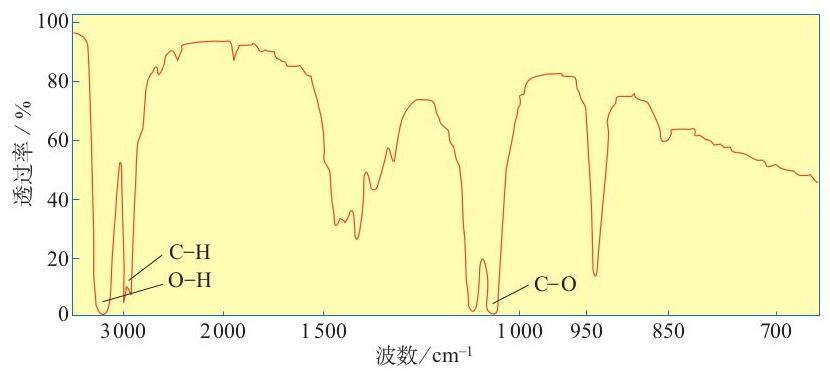
\includegraphics[max width=0.7\textwidth]{image/c75-1.jpg}
\end{center}

\subsection{质谱仪}

\textbf{原理}: 在质谱仪中使分子失去电子变成带正电荷的分子离子和碎片离子等粒子。由于生成的离子具有不同的相对质量, 他们在高压电场加速后, 通过狭缝进入磁场得以分离, 在记录仪上呈现一系列峰。质谱图\textbf{\uwave{最右边}}(横坐标)的分子离子峰表示待测物质的\textbf{\uwave{相对分子质量}}。

\begin{center}
	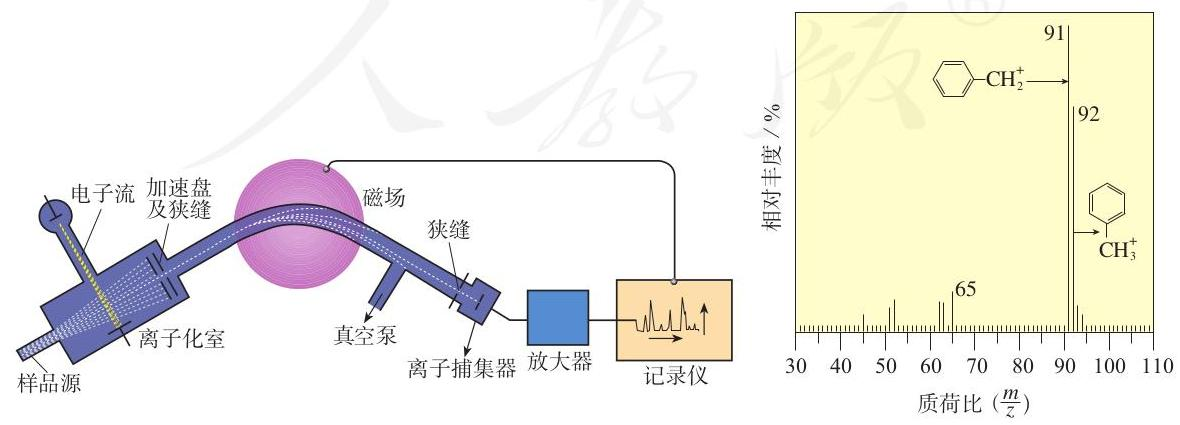
\includegraphics[max width=0.7\textwidth]{image/c75-2.jpg}
\end{center}

\section{价层电子对互斥模型 (VSEPR)}

只适用于$AB_{n}$

我们知道 \({\mathrm{{CO}}}_{2}\) 分子是直线形,而 \({\mathrm{H}}_{2}\mathrm{O}\) 分子是呈 \(\mathrm{V}\) 型。同样的三原子分子,空间结构却有很大的区别。为了预测分子的空间结构, 发展出了很多结构理论, 其中有一种比较简单的理论叫做价层电子对互斥模型 (VSEPR model)。

价层电子对互斥模型认为, 分子的空间结构是中心原子的“价层电子对”互相排斥的结果。

价层电子对: 中心原子的\textbf{ \(\sigma\) 键电子对} (共用)(单键、双键或三键都只算一个) 和中心原子的\textbf{孤电子对}(自己)。

$$ \text{中心原子的孤电子对数} = \frac{1}{2}\left( {a - {xb}}\right)$$

$$ \text{中心原子的价电子对数} = \text{中心原子的} \sigma \text{键电子对数} + \text{中心原子的孤电子对数}$$

其中: \(\mathrm{a}\) 为中心原子的价电子数 (即最外层电子数);

\(\mathrm{x}\) 为与中心原子结合的原子数目;

\(\mathrm{b}\) 为与中心原子结合的原子能接受的电子数 (即 8-最外层电子数, \(\mathrm{H}\) 为 1 )。


\begin{center}
	\adjustbox{max width=\textwidth}{
		\begin{tabular}{|c|c|}
			\hline
			分子 & \({\mathrm{{SO}}}_{2}\) \\
			\hline
			中心原子 & S \\
			\hline
			最外层电子数a & 6 \\
			\hline
			下角标n x & 2 \\
			\hline
			8-另一原子 b & 2 \\
			\hline
			中心原子的孤电子对数 & 1 \\
			\hline
			\(\sigma\) 键电子对数 & 2  \\
			\hline
			中心原子的价层电子对数 & 3  \\
			\hline
		\end{tabular}
	}
\end{center}

	价层电子对之间由于互相排斥, 各价层电子对会处在夹角尽可能大的位置上, 可得到含孤电子	对数的分子的 VSEPR 模型, 略去孤电子对可得到分子的空间构型。
	
	\begin{center}
		\adjustbox{max width=\textwidth}{
			\begin{tabular}{|c|c|c|c|c|}
				\hline
				中心原子价层电子对数 & VSEPR模型名称 & 孤电子对数 (排斥共用电子对) & 分子构型 & 键角 \\
				\hline
				2 & 直成型 & 0 & 直线型($CO_{2}$) & 1$80^{o}$\\
				\hline
				\multirow{2}{*}{3} & \multirow{2}{*}{平面三角形} & 0 & 平面三角形($AlCl_{3}$) & $120^{o} $\\
				\cline{3-5}
				& & 1 & V字形 & \(< {120}^{ \circ }\) \\
				\hline
				\multirow{3}{*}{4} & \multirow{3}{*}{正四面体} & 0 & 正四面体($CH_{4}$) & \({109}^{ \circ }{28}^{\prime }\) \\
				\cline{3-5}
				& & 1 & \({三角锥}\left( {N{H}_{3}}\right)\) & \(< {109}^{ \circ }\) \\
				\cline{3-5}
				& & 2 & \(V\) 字形($H_{2} O$) & <<$109^{ \circ }$ \\
				\hline
			\end{tabular}
		}
	\end{center}


由于孤电子对有较大斥力, 含孤电子对的分子的实测键角几乎都小于 VSEPR 模型的预测值。例如, \({\mathrm{H}}_{2}\mathrm{O}\) 的键角为 \({105}^{ \circ },{\mathrm{{NH}}}_{3}\) 的键角为 \({107}^{ \circ },{\mathrm{{NO}}}_{2}\) 的键角为 \({115}^{ \circ }\) 。

\textbf{速算价层电子对数}

$$\dfrac{\text{中心原子价电子数} + \text{配体给}e^{-} -\text{电荷}}{2}$$

配体给$e^{-}$

F,Cl,Br,I,H $\Rightarrow$ +1

O,S $\Rightarrow$0

N $\Rightarrow$-1

\section{杂化轨道理论}

1. 发现矛盾

甲烷的 4 个 \(\mathrm{C} - \mathrm{H}\) 单键都是 \(\sigma\) 键,然而,碳原子的 4 个价层原子轨道是 3 个相互垂直的 \(2\mathrm{p}\) 轨道和 1 个球形的 \(2\mathrm{\;s}\) 轨道,用它们和 4 个 \(\mathrm{H}\) 原子的 \(1\mathrm{\;s}\) 轨道重叠,不可能得到四个完全相同的 \(\mathrm{C} - \mathrm{H}\) 键, 也不可能得到正四面体形的甲烷分子。

2. 鲍林提出杂化轨道理论解决矛盾

杂化轨道理论是一种价键理论, 是鲍林为了解释分子的空间结构提出的。

杂化轨道理论的提出是一个发现矛盾并提出理论解释的过程。

当碳原子与 4 个氢原子形成甲烷分子时,碳原子的 \(2\mathrm{\;s}\) 轨道和 3 个 \(2\mathrm{p}\) 轨道会发生混杂,形成 4 个新的能量相同的、方向不同的轨道,各指向正四面体的 4 个顶角,夹角 \({109}^{ \circ }{28}^{\prime }\) ,称为 \({\mathrm{{sp}}}^{3}\) 杂化轨道。

当碳原子和 4 个氢原子结合时,碳原子的 4 个 \({\mathrm{{sp}}}^{3}\) 杂化轨道分别与 4 个氢原子的 \(1\mathrm{\;s}\) 轨道重叠, 形成 4 个 \(\mathrm{C} - \mathrm{H}\sigma\) 键,因此呈正四面体形的空间结构。

\begin{center}
	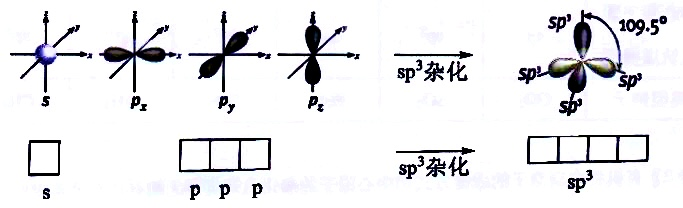
\includegraphics[max width=0.7\textwidth]{image/c83-1.jpg}
\end{center}

除了 \({\mathrm{{sp}}}^{3}\) 杂化轨道之外,还有 \(\mathrm{{sp}}\) 杂化轨道和 \({\mathrm{{sp}}}^{2}\) 杂化轨道。

\begin{center}
	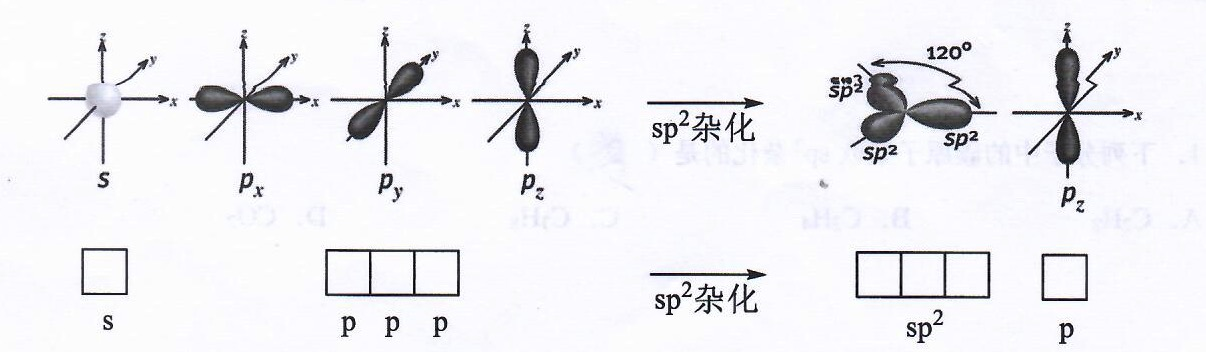
\includegraphics[max width=0.7\textwidth]{image/c83-2.jpg}
\end{center}

\begin{center}
	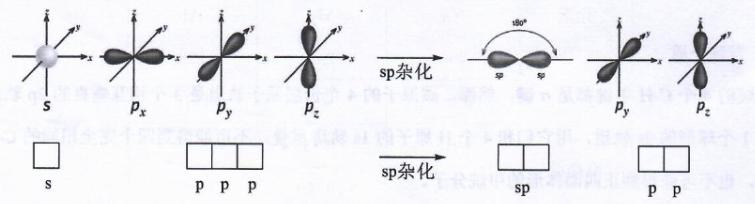
\includegraphics[max width=0.7\textwidth]{image/c84-1.jpg}
\end{center}
注意: 杂化轨道只用于形成 \(\sigma\) 键或用于容纳未参与成键的孤电子对


\begin{center}
	\adjustbox{max width=\textwidth}{
		\begin{tabular}{|c|c|c|c|c|c|c|}
			\hline
			VSEPR 模型 & 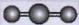
\includegraphics[max width=0.2\textwidth]{image/c84-2.jpg} & 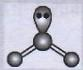
\includegraphics[max width=0.2\textwidth]{image/c84-3.jpg} & 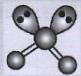
\includegraphics[max width=0.2\textwidth]{image/c84-4.jpg} & 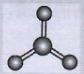
\includegraphics[max width=0.2\textwidth]{image/c84-5.jpg} & 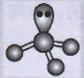
\includegraphics[max width=0.2\textwidth]{image/c84-6.jpg} & 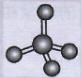
\includegraphics[max width=0.2\textwidth]{image/c84-7.jpg} \\
			\hline
			VSEPR 模型名称 & 直线形 & 平面三角 形 & 四面体 & 平面三角 形 & 四面体 & 正四面体 \\
			\hline
			中心原子杂 化轨道类型 & sp & \({\mathrm{{sp}}}^{2}\) & \({\mathrm{{sp}}}^{3}\) & \({\mathrm{{sp}}}^{2}\) & \({\mathrm{{sp}}}^{3}\) & \({\mathrm{{sp}}}^{3}\) \\
			\hline
			典型例子 & \({\mathrm{{CO}}}_{2}\) & \({\mathrm{{SO}}}_{2}\) & \({\mathrm{H}}_{2}\mathrm{O}\) & \({\mathrm{{SO}}}_{3}\) & \({\mathrm{{NH}}}_{3}\) & \({\mathrm{{CH}}}_{4}\) \\
			\hline
		\end{tabular}
	}
\end{center}

% 定义 longtable 环境,表格有 4 列,每列内容居中对齐并用竖线分隔
\begin{longtable}{|c|c|c|c|} 
	\hline % 表格顶部的横线
	
	% 表头部分
	价层电子对数 & 2 & 3 & 4 \\ % 表头行,加粗列标题
	\hline % 表头行的下横线
	\endfirsthead % 结束表头部分的定义
	
	% 表格主体的底部横线
	\hline
	\endfoot % 结束表格主体的底部横线部分
	
	% 表格最后一页的底部横线
	\hline
	\endlastfoot % 结束表格最后一页的底部横线部分
	
	% 表格内容部分
	杂化轨道类型& sp & $sp^{2}$& $sp^{3}$ \\ % 第一行数据
	\hline % 每行数据之后加横线

\end{longtable} % 结束 longtable 环境

有机物中都是单键 $\Rightarrow$ $sp^{3}$

有机物中有双键 $\Rightarrow$ $sp^{2}$

有机物中有三键/2个双键 $\Rightarrow$ $sp$


\chapter{分子结构与物质的性质}

\section{共价键的极性}

\textbf{极性共价键}: 由不同原子形成的共价键, 电子对会发生偏移, 是极性键, 极性键中的两个键合原子,一个呈正电性 \(\left( {\delta + }\right)\) ,另一个呈负电性 ( \(\delta -\) )。

\textbf{非极性共价键}: 电子对不发生偏移的共价键是非极性键。

\begin{center}
	\adjustbox{max width=\textwidth}{
		\begin{tabular}{|c|c|}
			\hline
			极性共价键 & 非极性共价键 \\
			\hline
			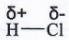
\includegraphics[max width=0.2\textwidth]{image/c88-1.jpg} & \(\mathrm{H} - \mathrm{H}\) \\
			\hline
			\(\mathrm{H}\) 的电负性小, \(\mathrm{{Cl}}\) 的电负性大 电子对偏向 \(\mathrm{{Cl}},\mathrm{H}\) 呈电正性, \(\mathrm{{Cl}}\) 呈电负性 & 两个 \(\mathrm{H}\) 原子的电负性相同 电子对不发生偏转 \\
			\hline
		\end{tabular}
	}
\end{center}

\textbf{极性分子}: 在极性分子中, 正电中心和负电中心不重合, 分子中各个键的极性向量和不为 0 , 使分子的某一个部分呈电正性 \(\left( {\delta + }\right)\) ,另一部分呈负电性 \(\left( {\delta - }\right)\) 。

\textbf{非极性分子}: 非极性分子的正电中心和负电中心重合, 分子中各个键的\textbf{\uwave{极性向量和}}等于 0 。

\begin{center}
	\adjustbox{max width=\textwidth}{
		\begin{tabular}{|c|c|}
			\hline
			极性分子 & 非极性分子 \\
			\hline
			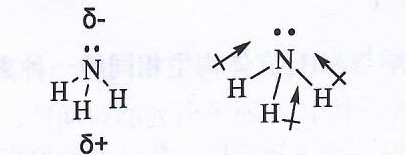
\includegraphics[max width=0.2\textwidth]{image/c88-3.jpg} & 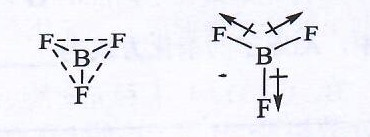
\includegraphics[max width=0.2\textwidth]{image/c88-4.jpg} \\
			\hline
			正电中心和负电中心不重合 & 正电中心和负电中心重合 \\
			\hline
			分子中各个键的极性向量和不为 \(0\) & 分子中各个键的极性向量和等于 \(0\) \\
			\hline
		\end{tabular}
	}
\end{center}

\textbf{\textit{单质分子不一定是非极性分子}}($O_{3}$)

$H_{2}O_{2}$\textit{不是平面结构}$\Rightarrow$极性

\subsection{羧酸的酸性}

键的极性对物质的化学性质有重要影响, 例如, 下表中羧酸的酸性。

\begin{center}
	\adjustbox{max width=\textwidth}{
		\begin{tabular}{|c|c|}
			\hline
			羧酸 & pKa (-lgKa)$\uparrow Ka \downarrow  $ 酸$\downarrow$ \\
			\hline
			丙酸( \({\mathrm{C}}_{2}{\mathrm{H}}_{5}\mathrm{{COOH}}\) ) & 4.88 \\
			\hline
			乙酸(CH3COOH) & 4.76 \\
			\hline
			甲酸(HCOOH) & 3.75 \\
			\hline
			氯乙酸(CH₂ClCOOH) & 2.86 \\
			\hline
			二氯乙酸(CHCl \({}_{2}\) COOH) & 1.29 \\
			\hline
			三氯乙酸(CCl \({}_{3}\) COOH) & 0.65 \\
			\hline
			三氟乙酸(CF3COOH) & 0.23 \\
			\hline
		\end{tabular}
	}
\end{center}

$$\text{电负性}\uparrow \text{极性}\uparrow  H^{+}\text{易出去}$$

\textit{吸电子集团(官能团)}$\uparrow$ 电负性$\uparrow$  O-H极性$\uparrow$  $H^{+}$ 易失去 $\Rightarrow$酸$\uparrow$ 

\textit{吸电子集团(R基)} C$\uparrow$ O-H极性$\downarrow$  $H^{+}$ 不易失去 $\Rightarrow$酸$\downarrow$ 
\subsection{无机酸酸性}

画结构式

键数目=|价态|

中心原子上\ce{=}O越多  O-H极性$\uparrow$   $\Rightarrow$酸性$\uparrow$ 

中心原子 电负性$\uparrow$  O-H极性$\uparrow$  $\Rightarrow$酸性$\uparrow$ 

\section{键参数——键能、键长与键角}

\subsection{键能 }


气态分子中 \(1\mathrm{\;{mol}}\) 化学键解离成气态原子所吸收的能量。

\textbf{键能的测量标准}: \({298.15}\mathrm{\;K}\text{、}{101}\mathrm{{kPa}}\) (常温常压下) 条件下。

\textbf{键能是一个平均值}: 键能可以通过实验测定, 但是更多的是通过推算得到的。化学键所处的化学环境不同,断开该化学键所需的能量也并不相同。比如断开 \({\mathrm{{CH}}}_{4}\) 中的 4 个 \(\mathrm{C} - \mathrm{H}\) 所需的能量并不相同,因此, \({\mathrm{{CH}}}_{4}\) 中的 \(\mathrm{C} - \mathrm{H}\) 键的键能是平均值。

\textbf{键能的作用}: 键能可用于估算化学反应的热效应。

\begin{center}
	\adjustbox{max width=\textwidth}{
		\begin{tabular}{|c|c|c|c|}
			\hline
			键 & 键能 kJ/mol & 键 & 键能 kJ/mol \\
			\hline
			\(\mathrm{H} - \mathrm{H}\) & 436.0 & \(\mathrm{N} \equiv \mathrm{N}\) & 946 \\
			\hline
			F-F & 157 & N-O & 176 \\
			\hline
			Cl-Cl & 242.7 & \(\mathrm{N} = \mathrm{O}\) & 607 \\
			\hline
			\(\mathrm{{Br}} - \mathrm{{Br}}\) & 193.7 & 0-0 & 142 \\
			\hline
			I-I & 152.7 & \(0 = 0\) & 497.3 \\
			\hline
			C-C & 347.7 & C-H & 413.4 \\
			\hline
			\(\mathrm{C} = \mathrm{C}\) & 615 & O-H & 462.8 \\
			\hline
			\(\mathrm{C} \equiv \mathrm{C}\) & 812 & \(\mathrm{N} - \mathrm{H}\) & 390.8 \\
			\hline
			C-O & 351 & \(\mathrm{H} - \mathrm{F}\) & 568 \\
			\hline
			\(\mathrm{C} = \mathrm{O}\) & 745 & H-Cl & 431.8 \\
			\hline
			\(\mathrm{N} - \mathrm{N}\) & 193 & \(\mathrm{H} - \mathrm{{Br}}\) & 366 \\
			\hline
			\(\mathrm{N} = \mathrm{N}\) & 418 & H-I & 298.7 \\
			\hline
		\end{tabular}
	}
\end{center}

\subsection{键长}

 构成化学键的两个原子的核间距。

\textbf{键长和键能的关系}: 当相同的两个原子形成共价键时, 一般情况下, \uwave{键长越小, 键能越大}(有例外,F-F<Cl-Cl<Br-Br<I-I)。比如 \(\mathrm{C} - \mathrm{C}\text{、}\mathrm{C} = \mathrm{C}\text{、}\mathrm{C} \equiv \mathrm{C}\) 的键长依次减小,键能依次增大

\begin{center}
	\adjustbox{max width=\textwidth}{
		\begin{tabular}{|c|c|c|c|}
			\hline
			键 & 键长 \(\mathrm{{pm}}\) & 键 & 键长 pm \\
			\hline
			\(\mathrm{H} - \mathrm{H}\) & 74 & \(\mathrm{C} \equiv \mathrm{C}\) & 120 \\
			\hline
			F-F & 141 & C-H & 109 \\
			\hline
			Cl-Cl & 198 & O-H & 96 \\
			\hline
			\(\mathrm{{Br}} - \mathrm{{Br}}\) & 228 & N-H & 101 \\
			\hline
			I-I & 267 & \(\mathrm{N} \equiv \mathrm{N}\) & 110 \\
			\hline
			C-C & 154 & Si-Si & 235 \\
			\hline
			\(\mathrm{C} = \mathrm{C}\) & 133 & Si-O & 162 \\
			\hline
		\end{tabular}
	}
\end{center}

\subsection{键角}

 在多原子分子中, 两个共价键之间的夹角称为键角。

多原子分子的键角一定, 说明共价键具有方向性。

常见分子的键角: \({\mathrm{{CO}}}_{2}{180}^{ \circ };{\mathrm{H}}_{2}\mathrm{O}{105}^{ \circ }\) ,因此 \({\mathrm{{CO}}}_{2}\) 是直线形分子, \({\mathrm{H}}_{2}\mathrm{O}\) 是 \(\mathrm{V}\) 型分子。

\textit{键角和键长的数值可以通过晶体的 \(\mathbf{X}\) \textbf{射线衍射实验}获得。}


\section{分子间的作用力}

\subsection{范德华力及其对物质性质的影响}

\textbf{范德华力}: 范德华最早研究分子间普遍存在作用力的科学家, 因而我们把这一类分子间作用力称为范德华力。

范德华力很弱, 比化学键的键能小 1~2 个数量级。\underline{相对分子质量越大, 范德华力越大; 分子极性越大, 范德华力也越大。}

\begin{center}
	\adjustbox{max width=\textwidth}{
		\begin{tabular}{|c|c|c|c|c|c|}
			\hline
			分子 & Ar & CO & \(\mathrm{{HI}}\) & \(\mathrm{{HBr}}\) & HCl \\
			\hline
			范德华力/kJ·mol- \({}^{1}\) & 8.50 & 8.75 & 26.00 & 23.11 & 21.14 \\
			\hline
		\end{tabular}
	}
\end{center}


\begin{center}
	\adjustbox{max width=\textwidth}{
		\begin{tabular}{|c|c|c|}
			\hline
			单质 & 熔点/℃ & 沸点 \(/{}^{ \circ }\mathrm{C}\) \\
			\hline
			\({\mathrm{F}}_{2}\) & -219.6 & -188.1 \\
			\hline
			\({\mathrm{{Cl}}}_{2}\) & -101 & -34.6 \\
			\hline
			\({\mathrm{{Br}}}_{2}\) & \(- {7.2}\) & 58.78 \\
			\hline
			\({\mathrm{I}}_{2}\) & 113.5 & 184.4 \\
			\hline
		\end{tabular}
	}
\end{center}


\subsection{ 氢键及其对物质性质的影响}

\textbf{氢键}: 氢键是除范德华力之外的另一种分子间作用力, 他是由已经与电负性很大的原子形成共价键的氢原子 (如水分子中的氢原子) 与另一个电负性很大的原子 (如水分子中的氧原子) 之间的作用力。氢键的存在, 大大加强了水分子之间的作用力, 所以水的熔、沸点较高。

氢键普遍存在于已经与 \(\mathrm{N}\text{、}\mathrm{O}\text{、}\mathrm{\;F}\) 等电负性很大的原子形成共价键的氢原子与另外的 \(\mathrm{N}\text{、}\mathrm{O}\text{、}\mathrm{\;F}\) 等电负性很大的原子之间。

\begin{center}
	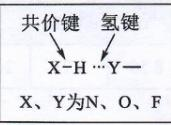
\includegraphics[max width=0.2\textwidth]{image/c96-1.jpg}
\end{center}

虽然我们把氢键也称为键, 但是与化学键相比, 氢键属于一种较弱的作用力, 比化学键的键能小 \(1 \sim 2\) 个数量级,不属于化学键。但是氢键的作用力一般比范德华力更大。

虽然氢键不是化学键, 但是其具有方向性和饱和性, 例如冰中水分子的氢键如下:

\begin{center}
	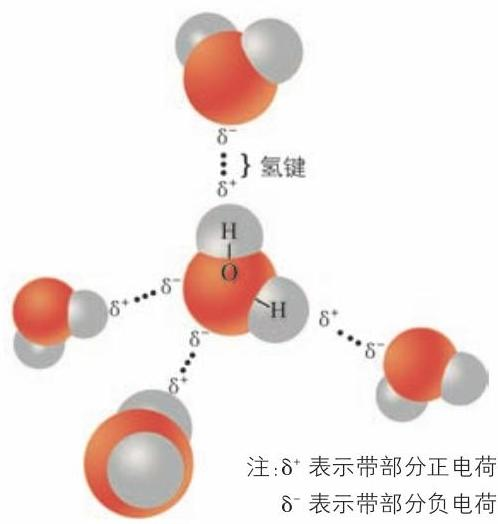
\includegraphics[max width=0.2\textwidth]{image/c96-2.jpg}
\end{center}

%【思考 4】观察下表卤素氢化物的熔沸点变化趋势, 并解释其原因。

\begin{center}
	\adjustbox{max width=\textwidth}{
		\begin{tabular}{|c|c|c|}
			\hline
			卤化氢 & 熔点/℃ & 沸点 \(/{}^{ \circ }\mathrm{C}\) \\
			\hline
			HF & -83.38 & 19.54 \\
			\hline
			\(\mathrm{{HCl}}\) & -114.2 & -85.0 \\
			\hline
			\(\mathrm{{HBr}}\) & -86.9 & -66.8 \\
			\hline
			HI & -50.8 & -35.1 \\
			\hline
		\end{tabular}
	}
\end{center}


\subsection{溶解性}



\textbf{相似相溶}: 非极性溶质一般能溶于非极性溶剂(有机), 极性溶质一般能溶于极性溶剂(H_{2}O)。

水是极性溶剂, 根据“相似相溶”, 极性溶质比非极性溶质在水中的溶解度大。

如果存在氢键, 则溶剂与溶质之间的氢键作用力越大, 溶解性越好。相反, 无氢键相互作用的溶质在有氢键的水中溶解度就比较小。

“相似相溶”还适用于分子结构的相似性。


\section{分子的手性}

\textbf{手性异构体}: 具有完全相同的组成和原子排列的一对分子, 如同左手和右手一样互为镜像, 但在三维空间内不能重合, 互称手性异构体 (或对映异构体)。有手性异构体的分子叫手性分子。

\begin{center}
	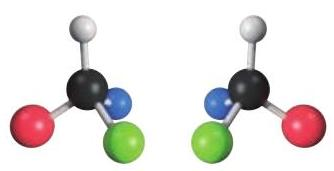
\includegraphics[max width=0.2\textwidth]{image/c102.jpg}
\end{center}

\textbf{常见的手性异构}: 当一个碳原子连接不同的四个基团的时候就会出现手性异构体。

\subsection{手性碳}

\textit{C原子上所连的4个基团各不相同}

\textit{无$\ce{=} /  \ce{#}$,至少连出去三根键}


%\section{晶体认识与类型}\\
\chapter{晶体认识与类型}

%自然界中绝大多数矿物都是固体。随着化学的发展, 人工合成的固体越来越多, 广泛应用于能源、 环境、材料、生命科学等领域。

\section{晶体与非晶体}

常见的固体分为\textbf{晶体}和\textbf{非晶体}, 以及介于晶体和非晶体之间的塑晶态、液晶态等。

绝大多数常见的固体是晶体, 只有如玻璃 (玻璃体)、炭黑 (无定形体) 之类的物质属于非晶体。 那么晶体和非晶体的本质差别是什么呢?

\textbf{晶体} (crystal): 是由大量微观粒子 (\underline{原子}、\underline{离子}、\underline{分子}等) 按\uwave{一定规则有序排列}的结构。


\textbf{非晶体}: 结构无序或者近程有序而长程无序的物质, 组成物质的分子 (或原子、离子) 不呈空间有规则周期性排列的固体。

\begin{center}
	\adjustbox{max width=\textwidth}{
		\begin{tabular}{|c|c|c|}
			\hline
			固体 & \uwave{自范性} & 微观结构 \\
			\hline
			晶体 & 有(能自发呈现多面体外形) & 微观粒子在三位空间里呈周期性有序排列 \\
			\hline
			非晶体 & 没有(不能自发呈现多面体外形) & 微观粒子排列相对无序 \\
			\hline
		\end{tabular}
	}
\end{center}

\subsection{自范性}

 粒子在微观空间里周期性有序排列必然会导致晶体在宏观上呈现出规则的外观。晶体能自发地呈现规则的多面体外形的性质称为晶体的自范性。

例如硫酸铜晶体能自发呈现规则的多面体外形, 而炭黑不能自发呈现规则的多面体结构。

晶体呈现自范性的条件之一是晶体的\uwave{生长速率适当}(溶液中析出)。熔融态物质冷却凝固, 有时得到晶体, 但凝固速率过快, 常常得到肉眼看不到多面体外形的粉末 (晶体颗粒很小) 或没有规则外形的块状物 (细小的晶体颗粒聚集在一起), 甚至形成的只是非晶态 (玻璃态)。

最有趣的例子是天然的水晶球。水晶球是岩浆里熔融态的 \({\mathrm{{SiO}}}_{2}\) 侵入地壳内的空洞冷却形成的。 剖开水晶球, 它的外层是看不到晶体外形的玛瑙, 内层才是呈现晶体外形的水晶。玛瑙是熔融的 \({\mathrm{{SiO}}}_{2}\) 快速冷却形成的,水晶是熔融态的 \({\mathrm{{SiO}}}_{2}\) 缓慢冷却形成的。

\subsection{各向异性}

 同一晶体格子中, 在不同的方向上质点的排列一般是不相同的 (例如下图中方向一和方向二), 晶体的物理性质, 如强度、导热性、光学性质等, 也随方向的不同而有所差异。这种差异称为晶体的各向异性。例如用一根红热的铁针刺中水晶柱面上凝固的石蜡, 石蜡在不同方向融化的快慢不同。

晶体的某些物理性质的各向异性也反映了晶体内部质点排列的有序性。


\begin{center}
	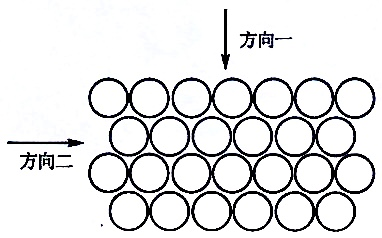
\includegraphics[max width=0.2\textwidth]{image/c106.jpg}
\end{center}

\subsection{均一性}

 同一晶体的各个部分质点分布是相同的, 所以同一晶体的各个部分的性质是相同的, 比如说同一晶体的熔点是固定的。所以可以通过确定某一固体的熔点是否固定来判断一个固体是否是晶体, 晶体有固定的熔点, 熔化过程中温度保持不变; 非晶体没有固定的熔点, 熔化过程中温度会发生变化。

\subsection{区分晶体和非晶体}

区分晶体和非晶体最可靠的科学方法是对固体进行 \(\mathbf{X}\) 射线衍射实验。

\(\mathrm{X}\) \textbf{射线衍射实验}: 当一束 \(\mathrm{X}\) 射线通过晶体时将发生衍射,衍射波叠加的结果使射线的强度在某些方向上加强,在其他方向上减弱。 \(\mathrm{X}\) 射线与晶体中的电子相互作用,会在记录仪上产生\textbf{分立的斑点或者明锐的衍射峰}。而在同一条件下摄取的非晶体图谱中却看不到分立的斑点或明锐的衍射峰。分析在照相底片上得到的衍射花样, 便可确定晶体结构。

\subsection{获得晶体的三大途径}

\ding{172} 熔融态物质凝固;

\ding{173} 气态物质冷却不经液态直接凝固 (凝华);

\ding{174} 溶质从溶液中析出。

\textbf{根据形成晶体的粒子以及作用力的不同, 我们将晶体分为分子晶体、共价晶体、金属晶体以及离子晶体四大类。}

\begin{center}
	\adjustbox{max width=\textwidth}{
		\begin{tabular}{|c|c|c|}
			\hline
			晶体类型 & 作用力 & 构成粒子 \\
			\hline
			分子晶体 & 分子间作用力 & 分子 \\
			\hline
			共价晶体 & 共价键 & 原子 \\
			\hline
			金属晶体 & 金属键 & 金属离子和电子 \\
			\hline
			离子晶体 & 离子键 & 阴阳离子 \\
			\hline
		\end{tabular}
	}
\end{center}

常见的晶体:

黄金(金属晶体)-金属,金刚石(共价晶体)-共价化合物,干冰(分子晶体)-共价化合物,萤石(离子晶体)-离子化合物

\begin{center}
	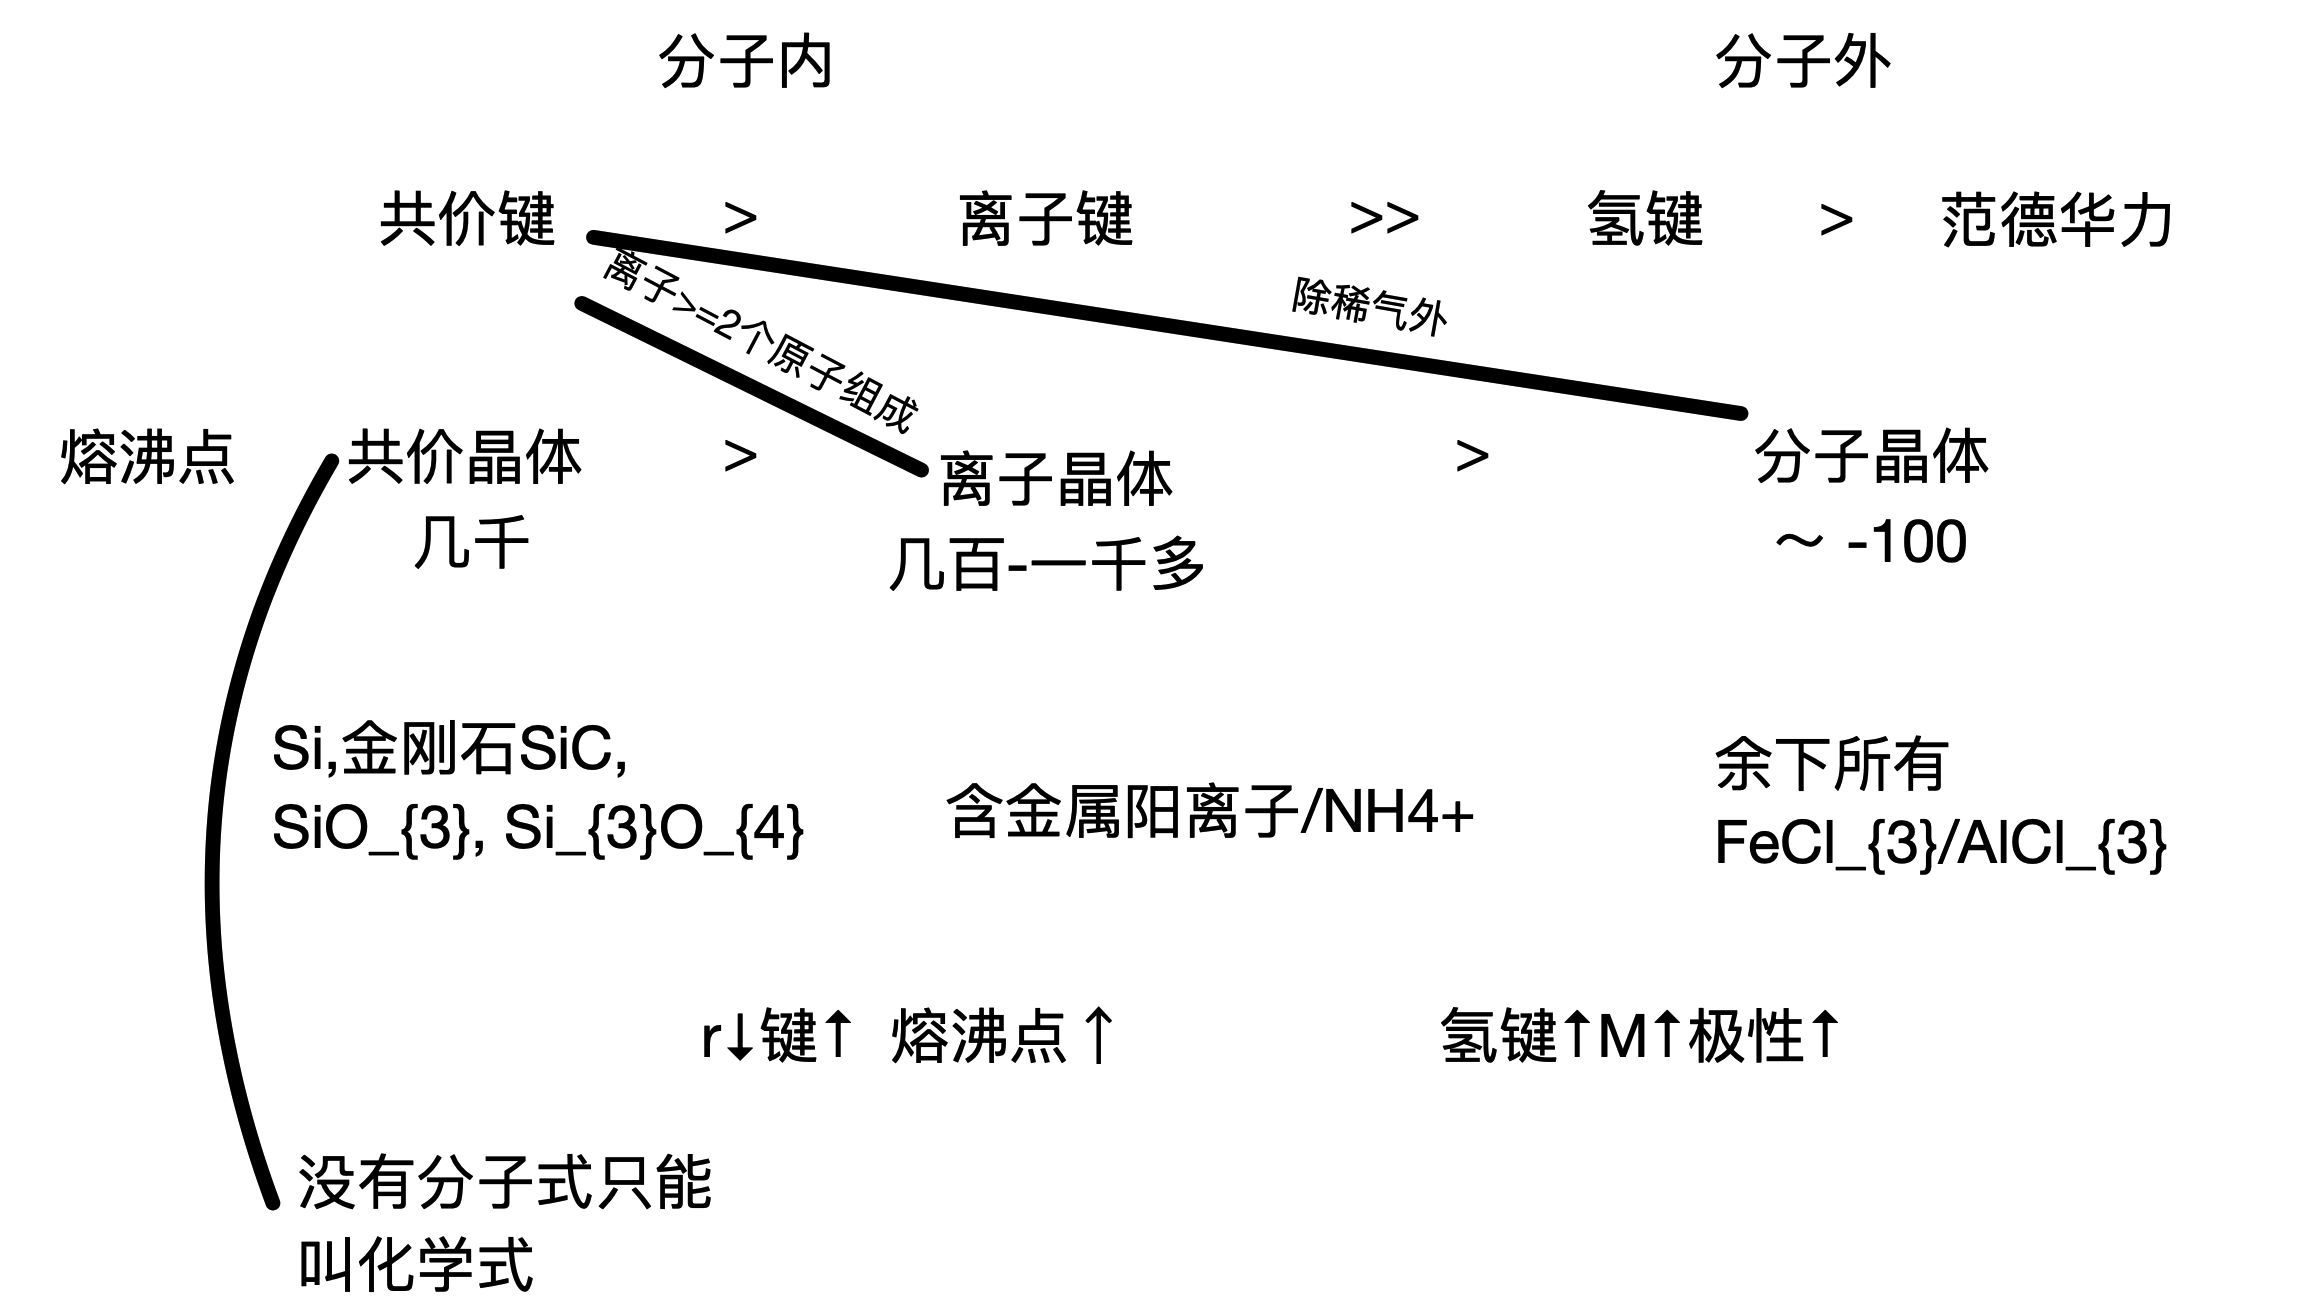
\includegraphics[max width=0.8\textwidth]{image/c109-2.jpg}
\end{center}

\section{分子晶体与分子间作用力}

\textbf{分子晶体特点}: 在分子晶体中, 相邻分子靠分子间作用力相互吸引。由于分子间作用力比较弱, 所以分子晶体有\textbf{低熔点、硬度小}的特性。

\begin{center}
	\adjustbox{max width=\textwidth}{
		\begin{tabular}{|c|c|c|c|c|}
			\hline
			分子晶体 & 氧气 & 氮气 & 白磷 & 水 \\
			\hline
			熔点/℃ & -218.3 & -210.1 & 44.2 & 0 \\
			\hline
			分子晶体 & 硫化氢 & 甲烷 & 乙酸 & 尿素 \\
			\hline
			熔点 \(/{}^{ \circ }\mathrm{C}\) & -85.6 & -182 & 16.6 & 132.7 \\
			\hline
		\end{tabular}
	}
\end{center}

某些分子晶体的熔点

分子晶体熔化或者升华过程中破坏分子间作用力 (范德华力或氢键)。例如干冰升华破坏范德华力, 冰熔化破坏氢键。

常见的分子晶体:

(1)所有的非金属氢化物:水、硫化氢、氨、甲烷等;

(2)部分非金属单质:卤素、氧气、硫( \({\mathrm{S}}_{8}\) )、氮气、白磷、碳 60 等;

(3)部分非金属氧化物: \({\mathrm{{CO}}}_{2}\text{、}{\mathrm{P}}_{4}{\mathrm{O}}_{6}\text{、}{\mathrm{P}}_{4}{\mathrm{O}}_{10}\text{、}{\mathrm{{SO}}}_{2}\) 等;

(4) 稀有气体

  (5) 几乎所有的酸;

(6)绝大多数有机物

\section{共价晶体与共价键}

\textbf{共价晶体特点}: 在共价晶体中, 相邻原子靠\textbf{共价键}相互吸引。\textbf{高硬度、高熔点}也是许多共价键三维骨架结构的共价晶体的特性。

\begin{center}
	\adjustbox{max width=\textwidth}{
		\begin{tabular}{|c|c|c|c|c|c|c|}
			\hline
			共价晶体 & 金刚石 & 氮化硼 & 碳化硅 & 石英 & 硅 & 锗 \\
			\hline
			熔点/℃ & 3900 & 3000 & 2700 & 1710 & 1410 & 1211 \\
			\hline
			硬度 & 10 & 9.5 & 9.5 & 7 & 6.5 & 6.0 \\
			\hline
		\end{tabular}
	}
\end{center}

常见的共价晶体还有

(1)某些单质, 如硼 (B)、硅 (Si)、锗 (Ge) 和灰锡 (Sn) 等;

(2)某些非金属化合物,如碳化硅(SiC,俗称金刚砂)、 \({\mathrm{{Si}}}_{3}{\mathrm{\;N}}_{4}\) 等。

近年来以 \({\mathrm{{Si}}}_{3}{\mathrm{\;N}}_{4}\) 为基础,用 \(\mathrm{{Al}}\) 取代部分 \(\mathrm{{Si}}\) ,用 \(\mathrm{O}\) 取代部分 \(\mathrm{N}\) 而获得结构多样化的陶瓷,用于制作 LED 发光材料。

\section{金属晶体与金属键}

\subsection{金属键}

 金属位于元素周期表的左部和中部, 非金属位于元素周期表的右部, 所以金属原子半径都比较大, 价电子数目少, 其电离能、电负性都比较低, 与非金属原子相比, 原子核对其本身价电子或其他原子的电子吸引力都比较弱, 表明金属较易失去电子, 这些脱离原子核的电子成为自由电子或离域电子。

\subsection{电子气理论}

 在固态或液态金属中, 金属原子的价电子成为“自由电子”, 在金属原子之间自由流动, 称为“自由电子气”, \textbf{金属离子}沉浸在“自由电子气”中。这种由自由电子的不停运动, 把金属离子连在一起的结合力, 称为\textbf{金属键}。

\begin{center}
	\includegraphics[max width=0.3\textwidth]{image/c115.jpg}
\end{center}

为了价电子云得到最大程度的重叠, 在金属晶体中金属原子间尽可能地最紧密排列, 使之占有最小空间, 得到稳定的金属晶体。由此可见, 金属晶体是一种“\textbf{巨分子}”。

\subsection{金属晶体}

 金属 (除汞外) 在常温下都是晶体。

\textbf{金属晶体特点}: 金属键的强度差别很大。

例: 金属钠的熔点较低、硬度较小, 而钨是熔点最高的金属、铬是硬度最大的金属, 这是由于形成的金属键强弱不同的缘故。


金属键的模型可以解释金属晶体的一些通性:

(1)由于金属中存在“自由电子”, 所以在外电场的作用下, “自由电子”朝一定方向运动, 产生电流, 即金属在固态或液态都有导电性。加热时, 金属离子振动加强, 阻碍“自由电子”的运动, 因而金属的电阻随温度升高而增大。

\begin{center}
	\includegraphics[max width=0.3\textwidth]{image/c116-1.jpg}
\end{center}

(2)当金属晶体受外力发生形变时, 虽然层与层之间的原子发生了相对位移, 由于“自由电子”的连接作用没有变化, 即金属键没有受到破坏, 金属晶体仍然存在, 只是被压扁、拉长, 这就是金属晶体具有延展性的原因。

\begin{center}
	\includegraphics[max width=1.0\textwidth]{image/c116-2.jpg}
\end{center}

电子气理论对金属延展性的解释

当向金属晶体中掺入不同的金属或非金属原子时, 会使这种金属的延展性甚至硬度发生改变。

(3)在金属晶体中“自由电子”很容易成为激发态“自由电子”, 所以它们可以吸收可见光, 而且把各种波长的光很大部分发射出去, 故绝大多数金属呈银白色光泽。

\section{离子晶体与离子键}

离子晶体: 由阳离子和阴离子相互作用而形成的晶体。

离子晶体特点: 离子间存在着较强的离子键, 使晶体的硬度较大, 难以压缩; 而且要使它们由固态变成液态和气态, 需要较多的能量破坏这些较强的离子键, 因此离子晶体有较高的熔沸点。

离子键是阴阳离子之间的静电作用, 因此离子的半径越小、带电量越大, 离子键的强度也越大, 离子晶体的晶格能越大, 熔沸点也越高。

\subsection{晶格能}

 在标准状况下,使 \(1\mathrm{\;{mol}}\) 离子晶体变成气态正离子和气态负离子时所吸收的能量。
 
 \chapter{晶胞}
 
 最小重复单元
 
 复制粘贴可形成所给图像

 \section{一维无限结构}
 
 一些大型分子可以在一维方向上有序延伸, 为了描述该分子的结构, 无需画出整个分子所有的原子, 只需要在分子链上取一个基本单元即可。
 
 例如在可降解塑料聚乳酸分子中我们可以取一个最小的重复出现的单元来表示聚乳酸。
 
 \begin{center}
 	\includegraphics[max width=0.8\textwidth]{image/c121-1.jpg}
 \end{center}
 
 \begin{center}
 \includegraphics[max width=0.6\textwidth]{image/c121-2.jpg}
 \end{center}
 
 再例如由硅氧四面体组成的硅酸盐长链。我们也可以取一个最小的重复出现的单元来表示硅酸跟离子 (一个 四面体的顶点为 O原子,体心为 \(\mathrm{{Si}}\) 原子)。
 
 \begin{center}
	\includegraphics[max width=0.8\textwidth]{image/c121-3.jpg}
\end{center}
 
 上述硅酸跟离子可以表示为 \({\left( {\mathrm{{Si}}}_{6}{\mathrm{O}}_{17}\right) }_{\mathrm{n}}{}^{{10}\mathrm{n} - }\) 。
 
 
 
 \section{二维无限结构}
 
 一些分子可以在二维方向上有序延伸。
 
 例如我们从石墨中撕下其中的一层得到的石墨烯就是一个二维延伸结构。
 
 
\begin{center}
	\includegraphics[max width=0.8\textwidth]{image/c123.jpg}
\end{center}
 
 我们从石墨烯中找到一个最小的结构单元, 整个石墨烯可以由这样\uwave{\textbf{完全等同}的结构单元\textbf{无隙并置而成}}。
 
\textbf{ 完全等同}: 结构单元的形状、取向、大小以及原子的种类、数目、排列完全相同。
 
\textbf{ 无隙并置}: 从一个结构单元仅通过平移就能和其他结构单元重合, 且各结构单元之间紧密排列没有空隙。
 
 
 \section{三维无限结构(晶体)}
 
 $\Rightarrow$共用,立方体
 
 为了描述晶体在微观空间里原子的排列, 无须画出千千万万个原子, 只需在晶体微观空间里取出一个基本单元即可。这种描述晶体结构的基本单元叫做晶胞。
 
 常规的晶胞, 都是平行六面体, 整块晶体是由完全等同的晶胞无隙并置地堆积而成的。
 
 \begin{center}
 	\includegraphics[max width=0.6\textwidth]{image/c125-2.jpg}
 \end{center}
 
 例如在铜晶体中, 取出一个一个重复出现的最小结构单元, 这个重复出现的结构单元就是铜晶胞,
 
 整个铜晶体由完全等同的铜晶胞无隙并置地堆积而成。
 
 在晶胞中,顶点的原子是被 8 个晶胞所共用的,所以每个晶胞实际只占有该原子的 \(\frac{1}{8}\) ;
 
 而棱上的原子被 4 个晶胞共用,所以每个晶胞实际只占有该原子的 \(\frac{1}{4}\) ;
 
 面上的原子被两个晶胞所共用,所以每个晶胞实际只占有该原子的 \(\frac{1}{2}\) ;
 
 内部的原子没有和其他晶胞共用, 所以每个晶胞占有一整个该原子。
 
 体心=总球数-已算的
 
 在晶胞的平行六面体中, 晶胞的 8 个顶点是完全相同的, 三套各 4 根平行棱分别相同, 三套各两个平行面分别相同。
 
 
 \section{常见物质的晶胞}
 
 \subsection{二氧化碳与分子晶体}
 
 二氧化碳是典型的分子晶体, 二氧化碳分子之间通过范德华力相互吸引结合形成的晶体。范德华力没有方向性, 如果将二氧化碳分子简化成球体, 那么在三维空间中, 二氧化碳分子在范德华力的作用下, 实现密堆积。
 
 若以一个二氧化碳分子为中心, 其周围通过分子间作用力与该分子紧密结合的分子总过有 12 个,
 
 即\textbf{配位数为 12 。}
 
\subsubsection{配位数}

 在晶体结构中某质点周围与该质点直接联系的质点数, 称为该质点的配位数。
 
 \textit{某质点离它最近的原子(另一种)有几个}
 
 \subsubsection{面心立方晶胞}
 
 我们可以从密堆积的二氧化碳分子晶体中可以得到如图所示的晶胞。可以看到, 二氧化碳分子占据晶胞的顶点和面心位置, 我们称这样的晶胞为\textbf{面心立方晶胞}。
 
\textit{ 只有顶点和面心}
 
 配位数12
 
 \subsection{氢键与冰晶体}
 
 如果分子间存在氢键, 例如我们熟悉的冰, 水分子之间主要的作用力是氢键。氢键虽然比化学键要弱的多, 不是化学键, 但是氢键也存在\textbf{方向性和饱和性}。所以在冰晶体中, 四面体中心的水分子只和四面体四个顶角的水分子相互吸引, 即配位数为 4 。
 
  \begin{center}
 	\includegraphics[max width=0.6\textwidth]{image/c129.jpg}
 \end{center}
 
 \subsection{金刚石与共价晶体}
 
 原子以具有方向性、饱和性的共价键为骨架形成的晶体称为共价晶体。
 
常见的共价晶体
 


 
 
 \subsubsection{金刚石}
 
  
 金刚石是典型的共价晶体。天然的金刚石经常呈现规则多面体的外形, 从这种外形就可以想象在金刚石晶体中, 每个碳原子以四个共价单键对称地与相邻的 4 个碳原子结合, C-C-C 夹角为 \({109}^{ \circ }{28}^{\prime }\) ,即金刚石中的碳采取 \({\mathrm{{sp}}}^{3}\) 杂化轨道形成共价键三维骨架结构。
 
\textit{ 8个C原子配位数4}
 
\textit{ 每个C周围$4 \times \dfrac{1}{2} = 2 $ 根键}
 
 
 \subsubsection{石英}
 
 \({\mathrm{{SiO}}}_{2}\) 是自然界含量最高的固态二元氧化物,熔点 \({1713}^{ \circ }\mathrm{C}\) ,有很多种结构,最常见的是低温石英。 如遍布海滩河岸的黄沙、带状的石英矿脉、花岗石中的白色晶体、透明的水晶等等。
 
 低温石英的结构中有顶角相连的硅氧四面体形成螺旋上升的长链, 而没有封闭的环状结构, 这一结构决定了它具有手性, 被广泛用作压电材料, 比如制作石英手表。
 
 石英晶体中 \(\mathrm{{Si}}\) 原子位于晶胞的顶点和面心以及不相邻的小立方体的体心 (把晶胞切成 8 个小立方体)。氧原子位于每两个最近的硅原子之间。
 
 
 $SiO_{2}$
 
 
\textit{ Si配位数4}
 
\textit{ O配位数2}
 
\textit{ 每Si周围4个Si-O}
 

   \subsection{ 氯化钠与氯化铯}
   
 离子晶体是由阳离子和阴离子相互作用而形成的晶体, 离子键没有方向性, 离子在三维空间的排列堆积方式取决于离子的带电量和离子的大小, 离子的带电量和大小不同, 离子晶体的晶胞也不同。
 
 比如 \(\mathrm{{NaCl}}\) 和氯化铯两种离子晶体的晶胞:

\subsubsection{  $NaCl$}
  
  $Na^{+}$ 6

  $Cl^{-}$ 6
  
\subsubsection{$CsCl$}
  
 \textit{ 体心立方堆积}
  
  \textit{配位数8,8}
  
  在 \(\mathrm{{NaCl}}\) 和 \(\mathrm{{CsCl}}\) 晶体中,离子间存在着较强的离子键,使晶体的硬度较大,难以压缩; 而且要使它们由固态变成液态和气态, 需要较多的能量破坏这些较强的离子键。因此, \(\mathrm{{NaCl}}\) 和 \(\mathrm{{CsCl}}\) 具有较高的熔点和沸点,如 \(\mathrm{{NaCl}}\) 的熔点为 \({801}^{ \circ }\mathrm{C}\) ,沸点为 \({1413}^{ \circ }\mathrm{C};\mathrm{{CsCl}}\) 的熔点为 \({645}^{ \circ }\mathrm{C}\) ,沸点为 \({1290}^{ \circ }\mathrm{C}\) 。


\subsection{ 金属晶体}

金属晶体是金属阳离子和电子通过金属键相互结合形成的晶体, 金属键没有方向性, 不同的金属在三维空间的堆积方式也不同, 其晶胞也不同, 即使是同一金属在不同的条件下, 晶胞也可能不同。

例如金属铁单质的晶体在不同温度下有两种堆积方式, 晶胞分别如下图所示。体心立方晶胞和面心立方晶胞中实际含有的铁原子个数之比为\_\_\_。金属单质铜也采取面心立方的晶胞。

\subsection{$LaNi_{5}$六方晶胞}

\({\mathrm{{LaNi}}}_{5}\) 晶体中,我们可以按照规则选取一个平行六面体作为晶胞,也可以选取如下图所示的一个结构单元作为晶胞。

顶点$\times \dfrac{1}{6}$

面心$\times \dfrac{1}{2}$

底棱$\times \dfrac{1}{4}$

侧棱$\times \dfrac{1}{3}$


\section{过渡晶体和混合晶体}

\subsection{ 过渡晶体}

我们已经知道了晶体大致分为分子晶体、共价晶体、金属晶体和离子晶体等四类典型晶体。然而、 纯粹的典型晶体是不多的, 大多数晶体是它们之间的过渡晶体。

以离子晶体和共价晶体之间的过渡为例。在第三周期前几种元素的氧化物中, 化学键中离子键成分的百分数如下表。

\begin{center}
	\adjustbox{max width=\textwidth}{
		\begin{tabular}{|c|c|c|c|c|}
			\hline
			氧化物 & \({\mathrm{{Na}}}_{2}\mathrm{O}\) & \(\mathrm{{MgO}}\) & \({\mathrm{{Al}}}_{2}{\mathrm{O}}_{3}\) & \({\mathrm{{SiO}}}_{2}\) \\
			\hline
			离子键的百分数/\% & 62 & 50 & 41 & 33 \\
			\hline
		\end{tabular}
	}
\end{center}

表中的 4 种氧化物晶体中的化学键既不是纯粹的离子键, 也不是纯粹的共价键, 这些晶体既不是纯粹的离子晶体也不是纯粹的共价晶体, 只是离子晶体与共价晶体之间的过渡晶体。

偏向离子晶体的过渡晶体在许多性质上与纯粹的离子晶体接近, 因而通常当作离子晶体来处理, 与 \({\mathrm{{Na}}}_{2}\mathrm{O}\) 等。同样,偏向共价晶体的过渡晶体则当作共价晶体来处理,如 \({\mathrm{{Al}}}_{2}{\mathrm{O}}_{3}\text{、}{\mathrm{{SiO}}}_{2}\) 等。

\subsection{ 混合晶体}

石墨的碳原子呈 \({\mathrm{{sp}}}^{2}\) 杂化,形成六元并环结构。所以石墨晶体是层状结构。每个碳原子没有杂化的 \(\mathrm{p}\) 轨道相互平行且重叠,使 \(\mathrm{p}\) 轨道中的电子可以在整个碳原子平面中运动,因此石墨有导电性

石墨晶体的结构中,层内的碳原子的核间距为 \( {142}\mathrm{{pm}} \) ,层间碳原子的距离为 \( {335}\mathrm{{pm}} \) ,说明层间没有化学键相连, 是靠范德华力维系

像石墨这样的晶体, 我们成为混合晶体。
\end{document}